\documentclass{report}

%%%%%%%%%%%%%%%%%%%%%%%%%%%%%%%%%
% PACKAGE IMPORTS
%%%%%%%%%%%%%%%%%%%%%%%%%%%%%%%%%


\usepackage[tmargin=2cm,rmargin=1in,lmargin=1in,margin=0.85in,bmargin=2cm,footskip=.2in]{geometry}
\usepackage[T1]{fontenc}
\usepackage{amsmath,amsfonts,amsthm,amssymb}
\usepackage{multirow,array,float,tabularx,booktabs,caption,tabu,pgf,tikz,pgfplots,environ,longtable,titlesec,titling,qrcode,placeins,xcolor,nameref}
\pgfplotsset{compat=1.18}
\usepackage[inline]{enumitem}
\usepackage[varbb]{newpxmath}
\usepackage{xfrac}
\usepackage[makeroom]{cancel}
\usepackage{mathtools}
\usepackage{bookmark}
\usepackage{hyperref,theoremref,cleveref}
\usepackage{listings}
\hypersetup{
	pdftitle={Assignment},
	colorlinks=true, linkcolor=doc!90,
	bookmarksnumbered=true,
	bookmarksopen=true
}
\usepackage[most,many,breakable]{tcolorbox}
\usepackage{xcolor}
\usepackage{varwidth}
\usepackage{varwidth}
\usepackage{etoolbox}
%\usepackage{authblk}
\usepackage{nameref}
\usepackage{multicol,array}
\usepackage{tikz-cd}
\usepackage[ruled,vlined,linesnumbered]{algorithm2e}
\usepackage{comment} % enables the use of multi-line comments (\ifx \fi) 
\usepackage{import}
\usepackage{xifthen}
\usepackage{pdfpages}
\usepackage{transparent}
\usepackage{graphicx}

\renewcommand{\chaptername}{Question}
\newcommand\mycommfont[1]{\footnotesize\ttfamily\textcolor{blue}{#1}}
\SetCommentSty{mycommfont}
\newcommand{\incfig}[1]{%
    \def\svgwidth{\columnwidth}
    \import{./figures/}{#1.pdf_tex}
}

\usepackage{tikzsymbols}
% \renewcommand\qedsymbol{$\Laughey$}


%\usepackage{import}
%\usepackage{xifthen}
%\usepackage{pdfpages}
%\usepackage{transparent}


%%%%%%%%%%%%%%%%%%%%%%%%%%%%%%
% SELF MADE COLORS
%%%%%%%%%%%%%%%%%%%%%%%%%%%%%%



\definecolor{myg}{RGB}{56, 140, 70}
\definecolor{myb}{RGB}{45, 111, 177}
\definecolor{myr}{RGB}{199, 68, 64}
\definecolor{mytheorembg}{HTML}{F2F2F9}
\definecolor{mytheoremfr}{HTML}{00007B}
\definecolor{mylenmabg}{HTML}{FFFAF8}
\definecolor{mylenmafr}{HTML}{983b0f}
\definecolor{mypropbg}{HTML}{f2fbfc}
\definecolor{mypropfr}{HTML}{191971}
\definecolor{myexamplebg}{HTML}{F2FBF8}
\definecolor{myexamplefr}{HTML}{88D6D1}
\definecolor{myexampleti}{HTML}{2A7F7F}
\definecolor{mydefinitbg}{HTML}{E5E5FF}
\definecolor{mydefinitfr}{HTML}{3F3FA3}
\definecolor{notesgreen}{RGB}{0,162,0}
\definecolor{myp}{RGB}{197, 92, 212}
\definecolor{mygr}{HTML}{2C3338}
\definecolor{myred}{RGB}{127,0,0}
\definecolor{myyellow}{RGB}{169,121,69}


%%%%%%%%%%%%%%%%%%%%%%%%%%%%
% TCOLORBOX SETUPS
%%%%%%%%%%%%%%%%%%%%%%%%%%%%

\setlength{\parindent}{1cm}
%================================
% THEOREM BOX
%================================

\tcbuselibrary{theorems,skins,hooks}
\newtcbtheorem[number within=section]{Theorem}{Theorem}
{%
	enhanced,
	breakable,
	colback = mytheorembg,
	frame hidden,
	boxrule = 0sp,
	borderline west = {2pt}{0pt}{mytheoremfr},
	sharp corners,
	detach title,
	before upper = \tcbtitle\par\smallskip,
	coltitle = mytheoremfr,
	fonttitle = \bfseries\sffamily,
	description font = \mdseries,
	separator sign none,
	segmentation style={solid, mytheoremfr},
	label type = theorem
}
{th}

\tcbuselibrary{theorems,skins,hooks}
\newtcbtheorem[number within=chapter]{theorem}{Theorem}
{%
	enhanced,
	breakable,
	colback = mytheorembg,
	frame hidden,
	boxrule = 0sp,
	borderline west = {2pt}{0pt}{mytheoremfr},
	sharp corners,
	detach title,
	before upper = \tcbtitle\par\smallskip,
	coltitle = mytheoremfr,
	fonttitle = \bfseries\sffamily,
	description font = \mdseries,
	separator sign none,
	segmentation style={solid, mytheoremfr},
	label type = theorem
}
{th}


\tcbuselibrary{theorems,skins,hooks}
\newtcolorbox{Theoremcon}
{%
	enhanced
	,breakable
	,colback = mytheorembg
	,frame hidden
	,boxrule = 0sp
	,borderline west = {2pt}{0pt}{mytheoremfr}
	,sharp corners
	,description font = \mdseries
	,separator sign none
}

%================================
% Corollery
%================================
\tcbuselibrary{theorems,skins,hooks}
\newtcbtheorem[number within=section]{Corollary}{Corollary}
{%
	enhanced
	,breakable
	,colback = myp!10
	,frame hidden
	,boxrule = 0sp
	,borderline west = {2pt}{0pt}{myp!85!black}
	,sharp corners
	,detach title
	,before upper = \tcbtitle\par\smallskip
	,coltitle = myp!85!black
	,fonttitle = \bfseries\sffamily
	,description font = \mdseries
	,separator sign none
	,segmentation style={solid, myp!85!black}
}
{th}
\tcbuselibrary{theorems,skins,hooks}
\newtcbtheorem[number within=chapter]{corollary}{Corollary}
{%
	enhanced
	,breakable
	,colback = myp!10
	,frame hidden
	,boxrule = 0sp
	,borderline west = {2pt}{0pt}{myp!85!black}
	,sharp corners
	,detach title
	,before upper = \tcbtitle\par\smallskip
	,coltitle = myp!85!black
	,fonttitle = \bfseries\sffamily
	,description font = \mdseries
	,separator sign none
	,segmentation style={solid, myp!85!black}
}
{th}


%================================
% LENMA
%================================

\tcbuselibrary{theorems,skins,hooks}
\newtcbtheorem[number within=section]{Lemma}{Lemma}
{%
	enhanced,
	breakable,
	colback = mylenmabg,
	frame hidden,
	boxrule = 0sp,
	borderline west = {2pt}{0pt}{mylenmafr},
	sharp corners,
	detach title,
	before upper = \tcbtitle\par\smallskip,
	coltitle = mylenmafr,
	fonttitle = \bfseries\sffamily,
	description font = \mdseries,
	separator sign none,
	segmentation style={solid, mylenmafr},
}
{th}

\tcbuselibrary{theorems,skins,hooks}
\newtcbtheorem[number within=chapter]{lemma}{Lemma}
{%
	enhanced,
	breakable,
	colback = mylenmabg,
	frame hidden,
	boxrule = 0sp,
	borderline west = {2pt}{0pt}{mylenmafr},
	sharp corners,
	detach title,
	before upper = \tcbtitle\par\smallskip,
	coltitle = mylenmafr,
	fonttitle = \bfseries\sffamily,
	description font = \mdseries,
	separator sign none,
	segmentation style={solid, mylenmafr},
}
{th}


%================================
% PROPOSITION
%================================

\tcbuselibrary{theorems,skins,hooks}
\newtcbtheorem[number within=section]{Prop}{Proposition}
{%
	enhanced,
	breakable,
	colback = mypropbg,
	frame hidden,
	boxrule = 0sp,
	borderline west = {2pt}{0pt}{mypropfr},
	sharp corners,
	detach title,
	before upper = \tcbtitle\par\smallskip,
	coltitle = mypropfr,
	fonttitle = \bfseries\sffamily,
	description font = \mdseries,
	separator sign none,
	segmentation style={solid, mypropfr},
}
{th}

\tcbuselibrary{theorems,skins,hooks}
\newtcbtheorem[number within=chapter]{prop}{Proposition}
{%
	enhanced,
	breakable,
	colback = mypropbg,
	frame hidden,
	boxrule = 0sp,
	borderline west = {2pt}{0pt}{mypropfr},
	sharp corners,
	detach title,
	before upper = \tcbtitle\par\smallskip,
	coltitle = mypropfr,
	fonttitle = \bfseries\sffamily,
	description font = \mdseries,
	separator sign none,
	segmentation style={solid, mypropfr},
}
{th}


%================================
% CLAIM
%================================

\tcbuselibrary{theorems,skins,hooks}
\newtcbtheorem[number within=section]{claim}{Claim}
{%
	enhanced
	,breakable
	,colback = myg!10
	,frame hidden
	,boxrule = 0sp
	,borderline west = {2pt}{0pt}{myg}
	,sharp corners
	,detach title
	,before upper = \tcbtitle\par\smallskip
	,coltitle = myg!85!black
	,fonttitle = \bfseries\sffamily
	,description font = \mdseries
	,separator sign none
	,segmentation style={solid, myg!85!black}
}
{th}




%================================
% EXAMPLE BOX
%================================

\newtcbtheorem[number within=section]{Example}{Example}
{%
	colback = myexamplebg
	,breakable
	,colframe = myexamplefr
	,coltitle = myexampleti
	,boxrule = 1pt
	,sharp corners
	,detach title
	,before upper=\tcbtitle\par\smallskip
	,fonttitle = \bfseries
	,description font = \mdseries
	,separator sign none
	,description delimiters parenthesis
}
{ex}

\newtcbtheorem[number within=chapter]{example}{Example}
{%
	colback = myexamplebg
	,breakable
	,colframe = myexamplefr
	,coltitle = myexampleti
	,boxrule = 1pt
	,sharp corners
	,detach title
	,before upper=\tcbtitle\par\smallskip
	,fonttitle = \bfseries
	,description font = \mdseries
	,separator sign none
	,description delimiters parenthesis
}
{ex}

%================================
% DEFINITION BOX
%================================

\newtcbtheorem[number within=section]{Definition}{Definition}{enhanced,
	before skip=2mm,after skip=2mm, colback=red!5,colframe=red!80!black,boxrule=0.5mm,
	attach boxed title to top left={xshift=1cm,yshift*=1mm-\tcboxedtitleheight}, varwidth boxed title*=-3cm,
	boxed title style={frame code={
					\path[fill=tcbcolback]
					([yshift=-1mm,xshift=-1mm]frame.north west)
					arc[start angle=0,end angle=180,radius=1mm]
					([yshift=-1mm,xshift=1mm]frame.north east)
					arc[start angle=180,end angle=0,radius=1mm];
					\path[left color=tcbcolback!60!black,right color=tcbcolback!60!black,
						middle color=tcbcolback!80!black]
					([xshift=-2mm]frame.north west) -- ([xshift=2mm]frame.north east)
					[rounded corners=1mm]-- ([xshift=1mm,yshift=-1mm]frame.north east)
					-- (frame.south east) -- (frame.south west)
					-- ([xshift=-1mm,yshift=-1mm]frame.north west)
					[sharp corners]-- cycle;
				},interior engine=empty,
		},
	fonttitle=\bfseries,
	title={#2},#1}{def}
\newtcbtheorem[number within=chapter]{definition}{Definition}{enhanced,
	before skip=2mm,after skip=2mm, colback=red!5,colframe=red!80!black,boxrule=0.5mm,
	attach boxed title to top left={xshift=1cm,yshift*=1mm-\tcboxedtitleheight}, varwidth boxed title*=-3cm,
	boxed title style={frame code={
					\path[fill=tcbcolback]
					([yshift=-1mm,xshift=-1mm]frame.north west)
					arc[start angle=0,end angle=180,radius=1mm]
					([yshift=-1mm,xshift=1mm]frame.north east)
					arc[start angle=180,end angle=0,radius=1mm];
					\path[left color=tcbcolback!60!black,right color=tcbcolback!60!black,
						middle color=tcbcolback!80!black]
					([xshift=-2mm]frame.north west) -- ([xshift=2mm]frame.north east)
					[rounded corners=1mm]-- ([xshift=1mm,yshift=-1mm]frame.north east)
					-- (frame.south east) -- (frame.south west)
					-- ([xshift=-1mm,yshift=-1mm]frame.north west)
					[sharp corners]-- cycle;
				},interior engine=empty,
		},
	fonttitle=\bfseries,
	title={#2},#1}{def}



%================================
% EXERCISE BOX
%================================

\makeatletter
\newtcbtheorem{question}{Question}{enhanced,
	breakable,
	colback=white,
	colframe=myb!80!black,
	attach boxed title to top left={yshift*=-\tcboxedtitleheight},
	fonttitle=\bfseries,
	title={#2},
	boxed title size=title,
	boxed title style={%
			sharp corners,
			rounded corners=northwest,
			colback=tcbcolframe,
			boxrule=0pt,
		},
	underlay boxed title={%
			\path[fill=tcbcolframe] (title.south west)--(title.south east)
			to[out=0, in=180] ([xshift=5mm]title.east)--
			(title.center-|frame.east)
			[rounded corners=\kvtcb@arc] |-
			(frame.north) -| cycle;
		},
	#1
}{def}
\makeatother

%================================
% SOLUTION BOX
%================================

\makeatletter
\newtcolorbox{solution}{enhanced,
	breakable,
	colback=white,
	colframe=myg!80!black,
	attach boxed title to top left={yshift*=-\tcboxedtitleheight},
	title=Solution,
	boxed title size=title,
	boxed title style={%
			sharp corners,
			rounded corners=northwest,
			colback=tcbcolframe,
			boxrule=0pt,
		},
	underlay boxed title={%
			\path[fill=tcbcolframe] (title.south west)--(title.south east)
			to[out=0, in=180] ([xshift=5mm]title.east)--
			(title.center-|frame.east)
			[rounded corners=\kvtcb@arc] |-
			(frame.north) -| cycle;
		},
}
\makeatother

%================================
% Question BOX
%================================

\makeatletter
\newtcbtheorem{qstion}{Question}{enhanced,
	breakable,
	colback=white,
	colframe=mygr,
	attach boxed title to top left={yshift*=-\tcboxedtitleheight},
	fonttitle=\bfseries,
	title={#2},
	boxed title size=title,
	boxed title style={%
			sharp corners,
			rounded corners=northwest,
			colback=tcbcolframe,
			boxrule=0pt,
		},
	underlay boxed title={%
			\path[fill=tcbcolframe] (title.south west)--(title.south east)
			to[out=0, in=180] ([xshift=5mm]title.east)--
			(title.center-|frame.east)
			[rounded corners=\kvtcb@arc] |-
			(frame.north) -| cycle;
		},
	#1
}{def}
\makeatother

\newtcbtheorem[number within=chapter]{wconc}{Wrong Concept}{
	breakable,
	enhanced,
	colback=white,
	colframe=myr,
	arc=0pt,
	outer arc=0pt,
	fonttitle=\bfseries\sffamily\large,
	colbacktitle=myr,
	attach boxed title to top left={},
	boxed title style={
			enhanced,
			skin=enhancedfirst jigsaw,
			arc=3pt,
			bottom=0pt,
			interior style={fill=myr}
		},
	#1
}{def}



%================================
% NOTE BOX
%================================

\usetikzlibrary{arrows,calc,shadows.blur,positioning,matrix,decorations.pathreplacing}
\tcbuselibrary{skins}
\newtcolorbox{note}[1][]{%
	enhanced jigsaw,
	colback=gray!20!white,%
	colframe=gray!80!black,
	size=small,
	boxrule=1pt,
	title=\textbf{Note:-},
	halign title=flush center,
	coltitle=black,
	breakable,
	drop shadow=black!50!white,
	attach boxed title to top left={xshift=1cm,yshift=-\tcboxedtitleheight/2,yshifttext=-\tcboxedtitleheight/2},
	minipage boxed title=1.5cm,
	boxed title style={%
			colback=white,
			size=fbox,
			boxrule=1pt,
			boxsep=2pt,
			underlay={%
					\coordinate (dotA) at ($(interior.west) + (-0.5pt,0)$);
					\coordinate (dotB) at ($(interior.east) + (0.5pt,0)$);
					\begin{scope}
						\clip (interior.north west) rectangle ([xshift=3ex]interior.east);
						\filldraw [white, blur shadow={shadow opacity=60, shadow yshift=-.75ex}, rounded corners=2pt] (interior.north west) rectangle (interior.south east);
					\end{scope}
					\begin{scope}[gray!80!black]
						\fill (dotA) circle (2pt);
						\fill (dotB) circle (2pt);
					\end{scope}
				},
		},
	#1,
}

%%%%%%%%%%%%%%%%%%%%%%%%%%%%%%
% SELF MADE COMMANDS
%%%%%%%%%%%%%%%%%%%%%%%%%%%%%%


\newcommand{\thm}[2]{\begin{Theorem}{#1}{}#2\end{Theorem}}
\newcommand{\mthm}[3]{\begin{Theorem}{#1}{#2}#3\end{Theorem}}
\newcommand{\cor}[2]{\begin{Corollary}{#1}{}#2\end{Corollary}}
\newcommand{\mlemma}[2]{\begin{Lemma}{#1}{}#2\end{Lemma}}
\newcommand{\mlma}[3]{\begin{Lemma}{#1}{#2}#3\end{Lemma}}
\newcommand{\mprop}[2]{\begin{Prop}{#1}{}#2\end{Prop}}
\newcommand{\clm}[3]{\begin{claim}{#1}{#2}#3\end{claim}}
\newcommand{\wc}[2]{\begin{wconc}{#1}{}\setlength{\parindent}{1cm}#2\end{wconc}}
\newcommand{\thmcon}[1]{\begin{Theoremcon}{#1}\end{Theoremcon}}
\newcommand{\ex}[2]{\begin{Example}{#1}{}#2\end{Example}}
\newcommand{\dfn}[2]{\begin{Definition}[colbacktitle=red!75!black]{#1}{}#2\end{Definition}}
\newcommand{\dfnc}[2]{\begin{definition}[colbacktitle=red!75!black]{#1}{}#2\end{definition}}
\newcommand{\qs}[2]{\begin{question}{#1}{}#2\end{question}}
\newcommand{\pf}[2]{\begin{myproof}[#1]#2\end{myproof}}
\newcommand{\nt}[1]{\begin{note}#1\end{note}}

\newcommand\Myperm[2][^n]{\prescript{#1\mkern-2.5mu}{}{P_{#2}}}
\newcommand\Mycomb[2][^n]{\prescript{#1\mkern-0.5mu}{}{C_{#2}}}

\newcommand*\circled[1]{\tikz[baseline=(char.base)]{
		\node[shape=circle,draw,inner sep=1pt] (char) {#1};}}
\newcommand\getcurrentref[1]{%
	\ifnumequal{\value{#1}}{0}
	{??}
	{\the\value{#1}}%
}
\newcommand{\getCurrentSectionNumber}{\getcurrentref{section}}
\newenvironment{myproof}[1][\proofname]{%
	\proof[\bfseries #1: ]%
}{\endproof}
\newcounter{mylabelcounter}

\makeatletter
\newcommand{\setword}[2]{%
	\phantomsection
	#1\def\@currentlabel{\unexpanded{#1}}\label{#2}%
}
\makeatother




\tikzset{
	symbol/.style={
			draw=none,
			every to/.append style={
					edge node={node [sloped, allow upside down, auto=false]{$#1$}}}
		}
}


% deliminators
\DeclarePairedDelimiter{\abs}{\lvert}{\rvert}
\DeclarePairedDelimiter{\norm}{\lVert}{\rVert}

\DeclarePairedDelimiter{\ceil}{\lceil}{\rceil}
\DeclarePairedDelimiter{\floor}{\lfloor}{\rfloor}
\DeclarePairedDelimiter{\round}{\lfloor}{\rceil}

\newcommand\SetSymbol[1][]{\nonscript\:#1\vert\allowbreak\nonscript\:\mathopen{}}
\providecommand\given{} % to make it exist
\DeclarePairedDelimiterX\Set[1]\{\}{\renewcommand\given{\SetSymbol[\delimsize]}#1}


\newsavebox\diffdbox
\newcommand{\slantedromand}{{\mathpalette\makesl{d}}}
\newcommand{\makesl}[2]{%
\begingroup
\sbox{\diffdbox}{$\mathsurround=0pt#1\mathrm{#2}$}%
\pdfsave
\pdfsetmatrix{1 0 0.2 1}%
\rlap{\usebox{\diffdbox}}%
\pdfrestore
\hskip\wd\diffdbox
\endgroup
}
\newcommand{\dd}[1][]{\ensuremath{\mathop{}\!\ifstrempty{#1}{%
\slantedromand\@ifnextchar^{\hspace{0.2ex}}{\hspace{0.1ex}}}%
{\slantedromand\hspace{0.2ex}^{#1}}}}
\ProvideDocumentCommand\dv{o m g}{%
  \ensuremath{%
    \IfValueTF{#3}{%
      \IfNoValueTF{#1}{%
        \frac{\dd #2}{\dd #3}%
      }{%
        \frac{\dd^{#1} #2}{\dd #3^{#1}}%
      }%
    }{%
      \IfNoValueTF{#1}{%
        \frac{\dd}{\dd #2}%
      }{%
        \frac{\dd^{#1}}{\dd #2^{#1}}%
      }%
    }%
  }%
}
\providecommand*{\pdv}[3][]{\frac{\partial^{#1}#2}{\partial#3^{#1}}}
%  - others
\DeclareMathOperator{\Lap}{\mathcal{L}}
\DeclareMathOperator{\Var}{Var} % varience
\DeclareMathOperator{\Cov}{Cov} % covarience
\DeclareMathOperator{\E}{E} % expected

% Since the amsthm package isn't loaded

% I prefer the slanted \leq
\let\oldleq\leq % save them in case they're every wanted
\let\oldgeq\geq
\renewcommand{\leq}{\leqslant}
\renewcommand{\geq}{\geqslant}

% % redefine matrix env to allow for alignment, use r as default
% \renewcommand*\env@matrix[1][r]{\hskip -\arraycolsep
%     \let\@ifnextchar\new@ifnextchar
%     \array{*\c@MaxMatrixCols #1}}


%\usepackage{framed}
%\usepackage{titletoc}
%\usepackage{etoolbox}
%\usepackage{lmodern}


%\patchcmd{\tableofcontents}{\contentsname}{\sffamily\contentsname}{}{}

%\renewenvironment{leftbar}
%{\def\FrameCommand{\hspace{6em}%
%		{\color{myyellow}\vrule width 2pt depth 6pt}\hspace{1em}}%
%	\MakeFramed{\parshape 1 0cm \dimexpr\textwidth-6em\relax\FrameRestore}\vskip2pt%
%}
%{\endMakeFramed}

%\titlecontents{chapter}
%[0em]{\vspace*{2\baselineskip}}
%{\parbox{4.5em}{%
%		\hfill\Huge\sffamily\bfseries\color{myred}\thecontentspage}%
%	\vspace*{-2.3\baselineskip}\leftbar\textsc{\small\chaptername~\thecontentslabel}\\\sffamily}
%{}{\endleftbar}
%\titlecontents{section}
%[8.4em]
%{\sffamily\contentslabel{3em}}{}{}
%{\hspace{0.5em}\nobreak\itshape\color{myred}\contentspage}
%\titlecontents{subsection}
%[8.4em]
%{\sffamily\contentslabel{3em}}{}{}  
%{\hspace{0.5em}\nobreak\itshape\color{myred}\contentspage}



%%%%%%%%%%%%%%%%%%%%%%%%%%%%%%%%%%%%%%%%%%%
% TABLE OF CONTENTS
%%%%%%%%%%%%%%%%%%%%%%%%%%%%%%%%%%%%%%%%%%%

\usepackage{tikz}
\definecolor{doc}{RGB}{0,60,110}
\usepackage{titletoc}
\contentsmargin{0cm}
\titlecontents{chapter}[3.7pc]
{\addvspace{30pt}%
	\begin{tikzpicture}[remember picture, overlay]%
		\draw[fill=doc!60,draw=doc!60] (-7,-.1) rectangle (-0.3,.5);%
		\pgftext[left,x=-3.5cm,y=0.2cm]{\color{white}\Large\sc\bfseries Question\ \thecontentslabel};%
	\end{tikzpicture}\color{doc!60}\large\sc\bfseries}%
{}
{}
{\;\titlerule\;\large\sc\bfseries Page \thecontentspage
	\begin{tikzpicture}[remember picture, overlay]
		\draw[fill=doc!60,draw=doc!60] (2pt,0) rectangle (4,0.1pt);
	\end{tikzpicture}}%
\titlecontents{section}[3.7pc]
{\addvspace{2pt}}
{\contentslabel[\thecontentslabel]{2pc}}
{}
{\hfill\small \thecontentspage}
[]
\titlecontents*{subsection}[3.7pc]
{\addvspace{-1pt}\small}
{}
{}
{\ --- \small\thecontentspage}
[ \textbullet\ ][]

\titlecontents{chapter}[3.7pc]
{\addvspace{30pt}%
	\begin{tikzpicture}[remember picture, overlay]%
		\draw[fill=doc!60,draw=doc!60] (-7,-.1) rectangle (-0.3,.5);%
		\pgftext[left,x=-3.5cm,y=0.2cm]{\color{white}\Large\sc\bfseries Question\ \thecontentslabel};%
	\end{tikzpicture}\color{doc!60}\large\sc\bfseries}%
{}
{}
{\;\titlerule\;\large\sc\bfseries Page \thecontentspage
	\begin{tikzpicture}[remember picture, overlay]
		\draw[fill=doc!60,draw=doc!60] (2pt,0) rectangle (4,0.1pt);
	\end{tikzpicture}}%
\titlecontents{figure}[3.7pc]
{\addvspace{2pt}}
{\contentslabel[\thecontentslabel]{2pc}}
{}
{\hfill\small \thecontentspage}
[]

\makeatletter
\def\thischaptertitle{}\def\thischapternumber{}
\newtoggle{noFigs}

\apptocmd{\@chapter}{\gdef\thischaptertitle{#1}\gdef\thischapternumber{\thechapter}%
	\global\toggletrue{noFigs}}{}{}

\AtBeginDocument{%
	\AtBeginEnvironment{figure}{%
		\iftoggle{noFigs}{
			\addtocontents{lof}{\protect\contentsline {chapter}%
				{\protect\numberline {\thischapternumber} {\thischaptertitle}}{}{} }
			\global\togglefalse{noFigs}
		}{}
	}%
}

\renewcommand{\tableofcontents}{%
	\chapter*{%
	  \vspace*{-20\p@}%
	  \begin{tikzpicture}[remember picture, overlay]%
		  \pgftext[right,x=15cm,y=0.2cm]{\color{doc!60}\Huge\sc\bfseries \contentsname};%
		  \draw[fill=doc!60,draw=doc!60] (13,-.75) rectangle (20,1);%
		  \clip (13,-.75) rectangle (20,1);
		  \pgftext[right,x=15cm,y=0.2cm]{\color{white}\Huge\sc\bfseries \contentsname};%
	  \end{tikzpicture}}%
	\@starttoc{toc}}
\renewcommand{\listoffigures}{%
	\chapter*{%
	  \vspace*{-20\p@}%
	  \begin{tikzpicture}[remember picture, overlay]%
		  \pgftext[right,x=17cm,y=0.2cm]{\color{doc!60}\Huge\sc\bfseries \listfigurename};%
		  \draw[fill=doc!60,draw=doc!60] (13,-.75) rectangle (20,1);%
		  \clip (13,-.75) rectangle (20,1);
		  \pgftext[right,x=17cm,y=0.2cm]{\color{white}\Huge\sc\bfseries \listfigurename};%
	  \end{tikzpicture}}%
	\@starttoc{lof}}
\makeatother

\crefname{lemma}{Lemma}{Lemmas}
\crefname{theorem}{Theorem}{Theorem}

\definecolor{codegreen}{rgb}{0,0.6,0}
\definecolor{codegray}{rgb}{0.5,0.5,0.5}
\definecolor{codepurple}{rgb}{0.58,0,0.82}
\definecolor{backcolour}{rgb}{0.95,0.95,0.92}

\lstdefinestyle{mystyle}{
    backgroundcolor=\color{backcolour},   
    commentstyle=\color{codegreen},
    keywordstyle=\color{magenta},
    numberstyle=\tiny\color{codegray},
    stringstyle=\color{codepurple},
    basicstyle=\ttfamily\footnotesize,
    breakatwhitespace=false,         
    breaklines=true,                 
    captionpos=b,                    
    keepspaces=true,                 
    numbers=left,                    
    numbersep=5pt,                  
    showspaces=false,                
    showstringspaces=false,
    showtabs=false,                  
    tabsize=2
}

\lstset{style=mystyle}
\graphicspath{ {./Graphics/} }
\pretitle{%
	\begin{center}
		\LARGE
		
\includegraphics[width=0.8\textwidth]{sit-logo-primary}\\[\bigskipamount]
}
\posttitle{\end{center}}
\newcommand{\eps}{\epsilon}
\newcommand{\veps}{\varepsilon}
\newcommand{\ol}{\overline}
\newcommand{\ul}{\underline}
\newcommand{\wt}{\widetilde}
\newcommand{\wh}{\widehat}
\newcommand{\vocab}[1]{\textbf{\color{blue} #1}}
\providecommand{\half}{\frac{1}{2}}
\newcommand{\dang}{\measuredangle} %% Directed angle
\newcommand{\ray}[1]{\overrightarrow{#1}}
\newcommand{\seg}[1]{\overline{#1}}
\newcommand{\arc}[1]{\wideparen{#1}}
\DeclareMathOperator{\cis}{cis}
\DeclareMathOperator*{\lcm}{lcm}
\DeclareMathOperator*{\argmin}{arg min}
\DeclareMathOperator*{\argmax}{arg max}
\newcommand{\cycsum}{\sum_{\mathrm{cyc}}}
\newcommand{\symsum}{\sum_{\mathrm{sym}}}
\newcommand{\cycprod}{\prod_{\mathrm{cyc}}}
\newcommand{\symprod}{\prod_{\mathrm{sym}}}
\newcommand{\Qed}{\begin{flushright}\qed\end{flushright}}
\newcommand{\SolQed}{\begin{flushright}\(\blacksquare\)\end{flushright}}
\newcommand{\parinn}{\setlength{\parindent}{1cm}}
\newcommand{\parinf}{\setlength{\parindent}{0cm}}
% \newcommand{\norm}{\|\cdot\|}
\newcommand{\inorm}{\norm_{\infty}}
\newcommand{\opensets}{\{V_{\alpha}\}_{\alpha\in I}}
\newcommand{\oset}{V_{\alpha}}
\newcommand{\opset}[1]{V_{\alpha_{#1}}}
\newcommand{\lub}{\text{lub}}
\newcommand{\del}[2]{\frac{\partial #1}{\partial #2}}
\newcommand{\Del}[3]{\frac{\partial^{#1} #2}{\partial^{#1} #3}}
\newcommand{\deld}[2]{\dfrac{\partial #1}{\partial #2}}
\newcommand{\Deld}[3]{\dfrac{\partial^{#1} #2}{\partial^{#1} #3}}
\newcommand{\lm}{\lambda}
\newcommand{\uin}{\mathbin{\rotatebox[origin=c]{90}{$\in$}}}
\newcommand{\usubset}{\mathbin{\rotatebox[origin=c]{90}{$\subset$}}}
\newcommand{\lt}{\left}
\newcommand{\rt}{\right}
\newcommand{\bs}[1]{\boldsymbol{#1}}
\newcommand{\exs}{\exists}
\newcommand{\st}{\strut}
\newcommand{\dps}[1]{\displaystyle{#1}}

\newcommand{\sol}{\setlength{\parindent}{0cm}\textbf{\textit{Solution:}}\setlength{\parindent}{1cm} }
\newcommand{\solve}[1]{\setlength{\parindent}{0cm}\textbf{\textit{Solution: }}\setlength{\parindent}{1cm}#1 \SolQed}
\newenvironment{inference}{\FloatBarrier\begin{table*}[h]\begin{center}\begin{tabular}{rl}}{\end{tabular}\end{center}\end{table*}\FloatBarrier}
\lstMakeShortInline[columns=fixed]|
%From M275 "Topology" at SJSU
\newcommand{\id}{\mathrm{id}}
\newcommand{\taking}[1]{\xrightarrow{#1}}
\newcommand{\inv}{^{-1}}

%From M170 "Introduction to Graph Theory" at SJSU
\DeclareMathOperator{\diam}{diam}
\DeclareMathOperator{\ord}{ord}
\newcommand{\defeq}{\overset{\mathrm{def}}{=}}

%From the USAMO .tex files
\newcommand{\ts}{\textsuperscript}
\newcommand{\dg}{^\circ}
\newcommand{\ii}{\item}

% % From Math 55 and Math 145 at Harvard
% \newenvironment{subproof}[1][Proof]{%
% \begin{proof}[#1] \renewcommand{\qedsymbol}{$\blacksquare$}}%
% {\end{proof}}

\newcommand{\liff}{\leftrightarrow}
\newcommand{\lthen}{\rightarrow}
\newcommand{\opname}{\operatorname}
\newcommand{\surjto}{\twoheadrightarrow}
\newcommand{\injto}{\hookrightarrow}
\newcommand{\On}{\mathrm{On}} % ordinals
\DeclareMathOperator{\img}{im} % Image
\DeclareMathOperator{\Img}{Im} % Image
\DeclareMathOperator{\coker}{coker} % Cokernel
\DeclareMathOperator{\Coker}{Coker} % Cokernel
\DeclareMathOperator{\Ker}{Ker} % Kernel
\DeclareMathOperator{\rank}{rank}
\DeclareMathOperator{\Spec}{Spec} % spectrum
\DeclareMathOperator{\Tr}{Tr} % trace
\DeclareMathOperator{\pr}{pr} % projection
\DeclareMathOperator{\ext}{ext} % extension
\DeclareMathOperator{\pred}{pred} % predecessor
\DeclareMathOperator{\dom}{dom} % domain
\DeclareMathOperator{\ran}{ran} % range
\DeclareMathOperator{\Hom}{Hom} % homomorphism
\DeclareMathOperator{\Mor}{Mor} % morphisms
\DeclareMathOperator{\End}{End} % endomorphism

% Things Lie
\newcommand{\kb}{\mathfrak b}
\newcommand{\kg}{\mathfrak g}
\newcommand{\kh}{\mathfrak h}
\newcommand{\kn}{\mathfrak n}
\newcommand{\ku}{\mathfrak u}
\newcommand{\kz}{\mathfrak z}
\DeclareMathOperator{\Ext}{Ext} % Ext functor
\DeclareMathOperator{\Tor}{Tor} % Tor functor
\newcommand{\gl}{\opname{\mathfrak{gl}}} % frak gl group
\renewcommand{\sl}{\opname{\mathfrak{sl}}} % frak sl group chktex 6

% More script letters etc.
\newcommand{\SA}{\mathcal A}
\newcommand{\SB}{\mathcal B}
\newcommand{\SC}{\mathcal C}
\newcommand{\SF}{\mathcal F}
\newcommand{\SG}{\mathcal G}
\newcommand{\SH}{\mathcal H}
\newcommand{\OO}{\mathcal O}

\newcommand{\SCA}{\mathscr A}
\newcommand{\SCB}{\mathscr B}
\newcommand{\SCC}{\mathscr C}
\newcommand{\SCD}{\mathscr D}
\newcommand{\SCE}{\mathscr E}
\newcommand{\SCF}{\mathscr F}
\newcommand{\SCG}{\mathscr G}
\newcommand{\SCH}{\mathscr H}

% Mathfrak primes
\newcommand{\km}{\mathfrak m}
\newcommand{\kp}{\mathfrak p}
\newcommand{\kq}{\mathfrak q}

% number sets
\newcommand{\RR}[1][]{\ensuremath{\ifstrempty{#1}{\mathbb{R}}{\mathbb{R}^{#1}}}}
\newcommand{\NN}[1][]{\ensuremath{\ifstrempty{#1}{\mathbb{N}}{\mathbb{N}^{#1}}}}
\newcommand{\ZZ}[1][]{\ensuremath{\ifstrempty{#1}{\mathbb{Z}}{\mathbb{Z}^{#1}}}}
\newcommand{\QQ}[1][]{\ensuremath{\ifstrempty{#1}{\mathbb{Q}}{\mathbb{Q}^{#1}}}}
\newcommand{\CC}[1][]{\ensuremath{\ifstrempty{#1}{\mathbb{C}}{\mathbb{C}^{#1}}}}
\newcommand{\PP}[1][]{\ensuremath{\ifstrempty{#1}{\mathbb{P}}{\mathbb{P}^{#1}}}}
\newcommand{\HH}[1][]{\ensuremath{\ifstrempty{#1}{\mathbb{H}}{\mathbb{H}^{#1}}}}
\newcommand{\FF}[1][]{\ensuremath{\ifstrempty{#1}{\mathbb{F}}{\mathbb{F}^{#1}}}}
% expected value
\newcommand{\EE}{\ensuremath{\mathbb{E}}}
\newcommand{\charin}{\text{ char }}
\DeclareMathOperator{\sign}{sign}
\DeclareMathOperator{\Aut}{Aut}
\DeclareMathOperator{\Inn}{Inn}
\DeclareMathOperator{\Syl}{Syl}
\DeclareMathOperator{\Gal}{Gal}
\DeclareMathOperator{\GL}{GL} % General linear group
\DeclareMathOperator{\SL}{SL} % Special linear group

%---------------------------------------
% BlackBoard Math Fonts :-
%---------------------------------------

%Captital Letters
\newcommand{\bbA}{\mathbb{A}}	\newcommand{\bbB}{\mathbb{B}}
\newcommand{\bbC}{\mathbb{C}}	\newcommand{\bbD}{\mathbb{D}}
\newcommand{\bbE}{\mathbb{E}}	\newcommand{\bbF}{\mathbb{F}}
\newcommand{\bbG}{\mathbb{G}}	\newcommand{\bbH}{\mathbb{H}}
\newcommand{\bbI}{\mathbb{I}}	\newcommand{\bbJ}{\mathbb{J}}
\newcommand{\bbK}{\mathbb{K}}	\newcommand{\bbL}{\mathbb{L}}
\newcommand{\bbM}{\mathbb{M}}	\newcommand{\bbN}{\mathbb{N}}
\newcommand{\bbO}{\mathbb{O}}	\newcommand{\bbP}{\mathbb{P}}
\newcommand{\bbQ}{\mathbb{Q}}	\newcommand{\bbR}{\mathbb{R}}
\newcommand{\bbS}{\mathbb{S}}	\newcommand{\bbT}{\mathbb{T}}
\newcommand{\bbU}{\mathbb{U}}	\newcommand{\bbV}{\mathbb{V}}
\newcommand{\bbW}{\mathbb{W}}	\newcommand{\bbX}{\mathbb{X}}
\newcommand{\bbY}{\mathbb{Y}}	\newcommand{\bbZ}{\mathbb{Z}}

%---------------------------------------
% MathCal Fonts :-
%---------------------------------------

%Captital Letters
\newcommand{\mcA}{\mathcal{A}}	\newcommand{\mcB}{\mathcal{B}}
\newcommand{\mcC}{\mathcal{C}}	\newcommand{\mcD}{\mathcal{D}}
\newcommand{\mcE}{\mathcal{E}}	\newcommand{\mcF}{\mathcal{F}}
\newcommand{\mcG}{\mathcal{G}}	\newcommand{\mcH}{\mathcal{H}}
\newcommand{\mcI}{\mathcal{I}}	\newcommand{\mcJ}{\mathcal{J}}
\newcommand{\mcK}{\mathcal{K}}	\newcommand{\mcL}{\mathcal{L}}
\newcommand{\mcM}{\mathcal{M}}	\newcommand{\mcN}{\mathcal{N}}
\newcommand{\mcO}{\mathcal{O}}	\newcommand{\mcP}{\mathcal{P}}
\newcommand{\mcQ}{\mathcal{Q}}	\newcommand{\mcR}{\mathcal{R}}
\newcommand{\mcS}{\mathcal{S}}	\newcommand{\mcT}{\mathcal{T}}
\newcommand{\mcU}{\mathcal{U}}	\newcommand{\mcV}{\mathcal{V}}
\newcommand{\mcW}{\mathcal{W}}	\newcommand{\mcX}{\mathcal{X}}
\newcommand{\mcY}{\mathcal{Y}}	\newcommand{\mcZ}{\mathcal{Z}}



%---------------------------------------
% Bold Math Fonts :-
%---------------------------------------

%Captital Letters
\newcommand{\bmA}{\boldsymbol{A}}	\newcommand{\bmB}{\boldsymbol{B}}
\newcommand{\bmC}{\boldsymbol{C}}	\newcommand{\bmD}{\boldsymbol{D}}
\newcommand{\bmE}{\boldsymbol{E}}	\newcommand{\bmF}{\boldsymbol{F}}
\newcommand{\bmG}{\boldsymbol{G}}	\newcommand{\bmH}{\boldsymbol{H}}
\newcommand{\bmI}{\boldsymbol{I}}	\newcommand{\bmJ}{\boldsymbol{J}}
\newcommand{\bmK}{\boldsymbol{K}}	\newcommand{\bmL}{\boldsymbol{L}}
\newcommand{\bmM}{\boldsymbol{M}}	\newcommand{\bmN}{\boldsymbol{N}}
\newcommand{\bmO}{\boldsymbol{O}}	\newcommand{\bmP}{\boldsymbol{P}}
\newcommand{\bmQ}{\boldsymbol{Q}}	\newcommand{\bmR}{\boldsymbol{R}}
\newcommand{\bmS}{\boldsymbol{S}}	\newcommand{\bmT}{\boldsymbol{T}}
\newcommand{\bmU}{\boldsymbol{U}}	\newcommand{\bmV}{\boldsymbol{V}}
\newcommand{\bmW}{\boldsymbol{W}}	\newcommand{\bmX}{\boldsymbol{X}}
\newcommand{\bmY}{\boldsymbol{Y}}	\newcommand{\bmZ}{\boldsymbol{Z}}
%Small Letters
\newcommand{\bma}{\boldsymbol{a}}	\newcommand{\bmb}{\boldsymbol{b}}
\newcommand{\bmc}{\boldsymbol{c}}	\newcommand{\bmd}{\boldsymbol{d}}
\newcommand{\bme}{\boldsymbol{e}}	\newcommand{\bmf}{\boldsymbol{f}}
\newcommand{\bmg}{\boldsymbol{g}}	\newcommand{\bmh}{\boldsymbol{h}}
\newcommand{\bmi}{\boldsymbol{i}}	\newcommand{\bmj}{\boldsymbol{j}}
\newcommand{\bmk}{\boldsymbol{k}}	\newcommand{\bml}{\boldsymbol{l}}
\newcommand{\bmm}{\boldsymbol{m}}	\newcommand{\bmn}{\boldsymbol{n}}
\newcommand{\bmo}{\boldsymbol{o}}	\newcommand{\bmp}{\boldsymbol{p}}
\newcommand{\bmq}{\boldsymbol{q}}	\newcommand{\bmr}{\boldsymbol{r}}
\newcommand{\bms}{\boldsymbol{s}}	\newcommand{\bmt}{\boldsymbol{t}}
\newcommand{\bmu}{\boldsymbol{u}}	\newcommand{\bmv}{\boldsymbol{v}}
\newcommand{\bmw}{\boldsymbol{w}}	\newcommand{\bmx}{\boldsymbol{x}}
\newcommand{\bmy}{\boldsymbol{y}}	\newcommand{\bmz}{\boldsymbol{z}}

%---------------------------------------
% Scr Math Fonts :-
%---------------------------------------

\newcommand{\sA}{{\mathscr{A}}}   \newcommand{\sB}{{\mathscr{B}}}
\newcommand{\sC}{{\mathscr{C}}}   \newcommand{\sD}{{\mathscr{D}}}
\newcommand{\sE}{{\mathscr{E}}}   \newcommand{\sF}{{\mathscr{F}}}
\newcommand{\sG}{{\mathscr{G}}}   \newcommand{\sH}{{\mathscr{H}}}
\newcommand{\sI}{{\mathscr{I}}}   \newcommand{\sJ}{{\mathscr{J}}}
\newcommand{\sK}{{\mathscr{K}}}   \newcommand{\sL}{{\mathscr{L}}}
\newcommand{\sM}{{\mathscr{M}}}   \newcommand{\sN}{{\mathscr{N}}}
\newcommand{\sO}{{\mathscr{O}}}   \newcommand{\sP}{{\mathscr{P}}}
\newcommand{\sQ}{{\mathscr{Q}}}   \newcommand{\sR}{{\mathscr{R}}}
\newcommand{\sS}{{\mathscr{S}}}   \newcommand{\sT}{{\mathscr{T}}}
\newcommand{\sU}{{\mathscr{U}}}   \newcommand{\sV}{{\mathscr{V}}}
\newcommand{\sW}{{\mathscr{W}}}   \newcommand{\sX}{{\mathscr{X}}}
\newcommand{\sY}{{\mathscr{Y}}}   \newcommand{\sZ}{{\mathscr{Z}}}


%---------------------------------------
% Math Fraktur Font
%---------------------------------------

%Captital Letters
\newcommand{\mfA}{\mathfrak{A}}	\newcommand{\mfB}{\mathfrak{B}}
\newcommand{\mfC}{\mathfrak{C}}	\newcommand{\mfD}{\mathfrak{D}}
\newcommand{\mfE}{\mathfrak{E}}	\newcommand{\mfF}{\mathfrak{F}}
\newcommand{\mfG}{\mathfrak{G}}	\newcommand{\mfH}{\mathfrak{H}}
\newcommand{\mfI}{\mathfrak{I}}	\newcommand{\mfJ}{\mathfrak{J}}
\newcommand{\mfK}{\mathfrak{K}}	\newcommand{\mfL}{\mathfrak{L}}
\newcommand{\mfM}{\mathfrak{M}}	\newcommand{\mfN}{\mathfrak{N}}
\newcommand{\mfO}{\mathfrak{O}}	\newcommand{\mfP}{\mathfrak{P}}
\newcommand{\mfQ}{\mathfrak{Q}}	\newcommand{\mfR}{\mathfrak{R}}
\newcommand{\mfS}{\mathfrak{S}}	\newcommand{\mfT}{\mathfrak{T}}
\newcommand{\mfU}{\mathfrak{U}}	\newcommand{\mfV}{\mathfrak{V}}
\newcommand{\mfW}{\mathfrak{W}}	\newcommand{\mfX}{\mathfrak{X}}
\newcommand{\mfY}{\mathfrak{Y}}	\newcommand{\mfZ}{\mathfrak{Z}}
%Small Letters
\newcommand{\mfa}{\mathfrak{a}}	\newcommand{\mfb}{\mathfrak{b}}
\newcommand{\mfc}{\mathfrak{c}}	\newcommand{\mfd}{\mathfrak{d}}
\newcommand{\mfe}{\mathfrak{e}}	\newcommand{\mff}{\mathfrak{f}}
\newcommand{\mfg}{\mathfrak{g}}	\newcommand{\mfh}{\mathfrak{h}}
\newcommand{\mfi}{\mathfrak{i}}	\newcommand{\mfj}{\mathfrak{j}}
\newcommand{\mfk}{\mathfrak{k}}	\newcommand{\mfl}{\mathfrak{l}}
\newcommand{\mfm}{\mathfrak{m}}	\newcommand{\mfn}{\mathfrak{n}}
\newcommand{\mfo}{\mathfrak{o}}	\newcommand{\mfp}{\mathfrak{p}}
\newcommand{\mfq}{\mathfrak{q}}	\newcommand{\mfr}{\mathfrak{r}}
\newcommand{\mfs}{\mathfrak{s}}	\newcommand{\mft}{\mathfrak{t}}
\newcommand{\mfu}{\mathfrak{u}}	\newcommand{\mfv}{\mathfrak{v}}
\newcommand{\mfw}{\mathfrak{w}}	\newcommand{\mfx}{\mathfrak{x}}
\newcommand{\mfy}{\mathfrak{y}}	\newcommand{\mfz}{\mathfrak{z}}


\title{\Huge{INF1008}\\Data Structures \& Algorithms}
\author{\huge{Group 10}}
\date{}

\begin{document}

\maketitle
\newpage% or \cleardoublepage
% \pdfbookmark[<level>]{<title>}{<dest>}
\pdfbookmark[section]{\contentsname}{toc}
\tableofcontents
\listoffigures
\pagebreak
\chapter{}
\section{Problem Statement}
Implement the queue ADT using a Doubly linked list using any programming language. After the implementation, make use of the standard queue operations to implement the stack ADT\@. Clearly demonstrate the validity of your implementation through enough test cases. Evaluate the time complexity of the push, pop, empty and full operations.
\section{Requirements/Specification}
Users will have access to a container with behaviour akin to a stack, however in the background, the processes are done using a queue and its functions built upon a linked list structure. Users will have access to the standard stack functions - |push|, |pop|, |isEmpty| and |isFull| operations.
\section{User Guide}
An executable is provided, users can run the executable directly and follow the on-screen prompts, more in-depth details are provided in the Testing section.
\section{Structure/Design}
The stack as well as the underlying queue containers both have generic types built into the system. Thus, the same code can be re-used to store different types of data, including class objects, should the programmer wish to do that.

There are 3 classes utilised in this program, ``Node'', ``QueueADT'' and ``StackADT''. All 3 classes are template classes using typename |T|.
\subsection{Node}
\begin{figure}[H]
	\caption{Node Class Overview}
	\centering
	\label[fig]{fig:qn1_node}
	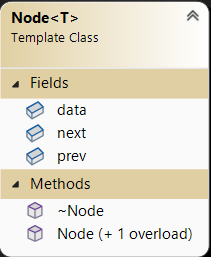
\includegraphics[height=0.25\textheight]{qn1_node}
\end{figure}
\begin{itemize}
	\item Data Members
	\begin{enumerate}
		\item |T data| -- Used to store the inputted data
		\item |Node<T>* next| -- Used to store the address of the next node, for use in a linked list
		\item |Node<T>* prev| -- Used to store the address of the previous node, for use in a linked list
	\end{enumerate}
	\item Methods
	\begin{enumerate}
		\item |Node()| -- Default constructor
		\item |~Node()| -- Default destructor
		\item |Node(T data)| -- An overloaded constructor, takes in a variable to initialise the data on construction.
	\end{enumerate}
\end{itemize}
\begin{figure}[H]
	\caption{Queue Class Overview}
	\centering
	\label[fig]{fig:qn1_queue}
	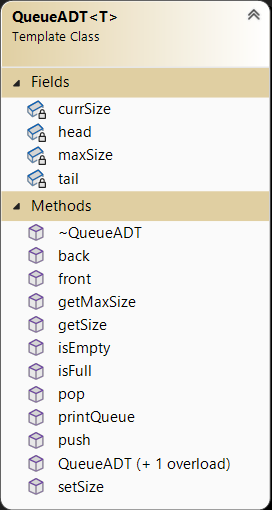
\includegraphics[height=0.25\textheight]{qn1_queue}
\end{figure}
\subsection{QueueADT}
\begin{itemize}
	\item Data Members
	\begin{enumerate}
		\item |int maxSize| -- Used to limit the size of the container
		\item |int currSize| -- Denotes the amount of data stored in the container, will be updated as the data is added and removed from the container
		\item |Node<T>* head| -- A pointer to the head node of the queue
		\item |Node<T>* tail| -- A pointer to the tail node of the queue
	\end{enumerate}
	\item Methods
	\begin{enumerate}
		\item |QueueADT()| -- Default constructor
		\item |~QueueADT()| -- Default destructor, will iterate through the linked list and delete all nodes when called
		\item |QueueADT(int size)| -- An overloaded constructor, takes an int argument to initialise |maxSize|
		\item |front()| -- Returns a pointer to the head node of the queue
		\item |back()| -- Returns a pointer to the tail node of the queue
		\item |setMaxSize(int size)| -- Passes in an integer to change the container's max allotted size
		\item |getMaxSize()| -- Returns |maxSize|
		\item |getSize()| -- Returns |currSize|
		\item |isEmpty()| -- Returns the truth value of |if currSize| equal to |0| and if |head| or |tail| are |NULL| as an added precaution, has a time complexity of \(\mathcal{O}(1)\) as |currSize| is updated together with the container, with the greater than or equal to comparator being used as an added precaution
		\item |isFull()| -- Returns the truth value of if |currSize| is greater than or equal to |maxSize|, has a time complexity of \(\mathcal{O}(1)\) as |currSize| is updated together with the container, with the greater than or equal to comparator being used as an added precaution.
		\item |push(T data)| -- |data| is passed in, and a |Node| is constructed using its overloaded constructor to be added to the linked list, as well as link the nodes between each other, has a time complexity of \(\mathcal{O}(1)\), as the pointer to the |tail| is stored, new elements can simply be added directly behind |tail| as no comparisons are required. Updates |currSize|, |head|, and |tail| members accordingly
		\item |pop()| -- Removes the element at the front of the queue, and returns a pointer to it to have its data extracted or deleted accordingly, has a time complexity of \(\mathcal{O}(1)\), as a pointer to |head| is stored, thus the front element can be removed directly with no comparisons. Updates |currSize|, |head|, and |tail| members accordingly
		\item |printQueue()| -- Prints the entire linked list, has a time complexity of \(\mathcal{O}(n)\) as iteration through the entire list is required
	\end{enumerate}
\end{itemize}
\subsection{StackADT}
\begin{figure}[H]
	\caption{Stack Class Overview}
	\centering
	\label[fig]{fig:qn1_stack}
	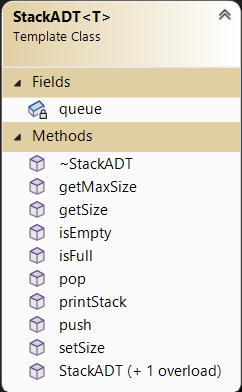
\includegraphics[height=0.25\textheight]{qn1_stack}
\end{figure}
\begin{itemize}
	\item Data Members
	\begin{enumerate}
		\item |QueueADT<T>* queue| -- A pointer to the queue container used to store data
	\end{enumerate}
	\item Methods
	\begin{enumerate}
		\item |StackADT()| -- Default constructor
		\item |~StackADT()| -- Default destructor, invokes the queue destructor, and deletes the pointer to the queue
		\item |StackADT(int size)| -- Overloaded constructor, initialises the |QueueADT| member with a |maxSize| of the value passed in
		\item |setMaxSize(int size)| -- Invokes the |QueueADT| member's |setMaxSize(int size)|, passing the same value in
		\item |getMaxSize()| -- Invokes the |QueueADT| member's |getMaxSize()|
		\item |getSize()| -- Invokes the |QueueADT| member's |getSize()|
		\item |isEmpty()| -- Invokes the |QueueADT| member's |isEmpty()|, therefore time complexity of \(\mathcal{O}(1)\)
		\item |isFull()| -- Invokes the |QueueADT| member's |isFull()|, therefore time complexity of \(\mathcal{O}(1)\)
		\item |push(T data)| -- Invokes the |QueueADT| member's |push(T data)|, after pushing the initial data in, all the other members in front of it are popped, and re-pushed into the queue to simulate a stack. This causes the function to have a time complexity of \(\mathcal{O}(n)\), as every element in the container has to be reorganised
		\item |pop()| -- Invokes the |QueueADT| member's |pop()|, therefore time complexity of \(\mathcal{O}(1)\)
	\end{enumerate}
\end{itemize}
\section{Limitations}
The data type specified on creation is final and is unable to be changed unless the stack is completely re-initialised. A consideration was made to utilise a class holding multiple data types - |int|(4 bytes), |float|(4 bytes), |double|(8 bytes), |char|(1 byte), |std::string|(\(>24\) bytes) - and construct a container with the type of that class. It would allow the container to store any data that has shares the property of being a standard data type. However, upon further deliberation, a class with that many types will cause memory bloat, as an example if the majority of the data entered was integers, for every 4 bytes used, \(>37\) bytes are reserved but unused by the system.
\section{Testing}
Users will be prompted (option 1 or option 2) to either allow the program to automatically generate test cases, or test the system out themselves. Users can also input a ``\$'' to terminate the program.
\begin{figure}[H]
	\centering
	\caption{Command-line Interface prompt}
	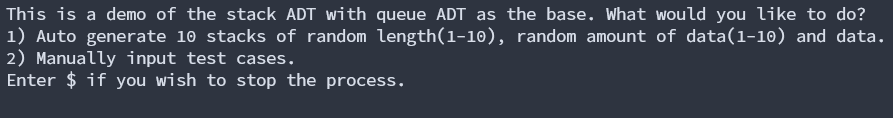
\includegraphics[width=0.8\textwidth]{qn1_input}
	\label{fig:qn1_prompt}
\end{figure}
\subsection{Option 1 -- Automatic Generation}
The program will prompt the user for the type of data they wish to store.
\begin{figure}[H]
	\centering
	\caption{Option 1 prompt}
	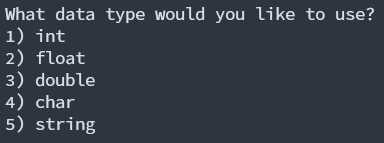
\includegraphics[width=0.8\textwidth]{qn1_option1}
	\label{fig:qn1_op1}
\end{figure}
The program will then generate 10 stacks of random length and random amount of data corresponding to the data type specified by the user.

\begin{figure}[H]
	\centering
	\caption{Option 1 testing}
	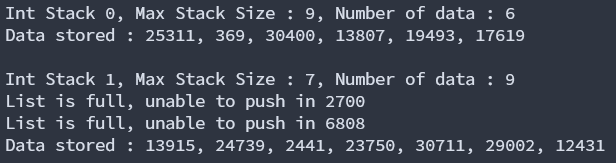
\includegraphics[width=0.8\textwidth]{qn1_op1_test}
	\label{fig:qn1_op1_test}
\end{figure}
\subsection{Option 2 -- Manual Testing}
The program will similarly prompt the user for the type of data they wish to store. Additionally, it will enquire on the size they wish for the container to be.

The user will then be able to enter data fitting to the data type into the stack, any data not fitting the data type will be rejected, discarding it and looping back to where the user can continue inputting data. Similarly, if the user tries to add more data into the stack when it is full, the program will also reject the entry. At any time the user can choose to enter ``\$'' and the process will end, and loop back to the start of the program.

\begin{figure}[H]
	\centering
	\caption{Option 2 testing with invalid inputs}
	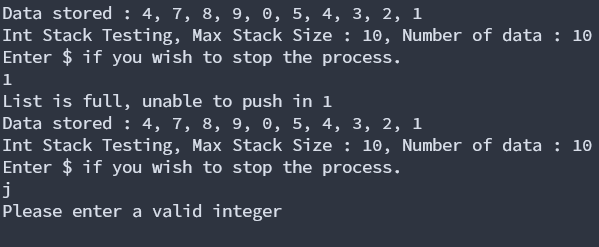
\includegraphics[width=0.8\textwidth]{qn1_op2}
	\label{fig:qn1_op2}
\end{figure}
\section{Listings}
\subsection{QueueADT.cpp}
\begin{lstlisting}[language=C++]
		
	#pragma once
	#include "QueueADT.h"

	template <class T>
	QueueADT<T>::QueueADT() {
		maxSize = 0;
		currSize = 0;
		head = tail = NULL;
	}

	template <class T>
	QueueADT<T>::QueueADT(int size) {
		maxSize = size;
		currSize = 0;
		head = tail = NULL;
	}

	//delete, could do the same thing as empty? 
	template <class T>
	QueueADT<T>::~QueueADT() {
		Node<T>* iter = head;
		//while iter exists, delete it and move next
		while (iter) {
			head = iter;
			iter = iter->next;
			delete head;
			head = NULL;
		}
		//safety
		head = tail = iter = NULL;
	}
	template <class T>
	void QueueADT<T>::setMaxSize(int size) {
		maxSize = size;
	}

	template <class T>
	int QueueADT<T>::getSize() {
		return currSize;
	}

	template <class T>
	int QueueADT<T>::getMaxSize() {
		return maxSize;
	}

	//insert element at the end of the Queuee
	template <class T>
	void QueueADT<T>::push(T data) {

		// if list is full return out
		if (isFull()) {
			std::cout << "Container full, failed to push "<< data << std::endl;
			return;
		}

		Node<T>* newNode = new Node<T>(data);

		//check if list is empty, if yes assign head and tail to same node 
		if (isEmpty()) {
			head = tail = newNode;	
			++currSize;
			return;
		}

		//getting last object and linking newNode to list
		Node<T>* iter = tail;
		iter->next = newNode;
		newNode->prev = iter;
		tail = newNode;
		++currSize; //add to counter
	}

	//remove and return 1st element
	template <class T>
	Node<T>* QueueADT<T>::pop() {
		if (isEmpty()) {
			return NULL;
		}
		Node<T>* iter = head;
		if (head->next != NULL) {
			head = head->next; //move head pointer back
		}
		head->prev = NULL; //break prev link to old head node
		iter->next = NULL; //break next link from old head node
		--currSize; //minus counter
		return iter;
	}

	//checks if container is empty
	template <class T>
	bool QueueADT<T>::isEmpty() {
		//returns if head and tail are both NULL
		return ((head == NULL || tail == NULL) && currSize == 0);
	}

	//returns if the Queuee is full / at capacity
	template <class T>
	bool QueueADT<T>::isFull() {
		return currSize >= maxSize;
	}

	template <class T>
	void QueueADT<T>::printQueue() {
		//if head or tail is not init, something wrong return out
		if (!head || !tail)
			return;

		std::cout << "Data stored : ";
		//printing data in list
		Node<T>* iter = head;
		while (iter != NULL) {
			//printf("%.6f", iter->data); //printf here to acheieve format
			std::cout << iter->data;
			//formatting
			if (iter->next != NULL)
				std::cout << ", ";
			iter = iter->next;
		}
		std::cout << std::endl;
	}

	template<class T>
	Node<T>* QueueADT<T>::front()
	{
		//if head exists return head else NULL
		if (head)
			return head;

		return NULL;
	}

	template<class T>
	Node<T>* QueueADT<T>::back()
	{
		//if tail exists return head else NULL
		if (tail)
			return tail;

		return NULL;
	}

\end{lstlisting}
\subsection{StackADT.cpp}
\begin{lstlisting}[language=C++]
	
	#pragma once
	#include "StackADT.h"

	template<class T>
	StackADT<T>::StackADT(){
		queue = new QueueADT<T>(0);
	}

	template<class T>
	StackADT<T>::StackADT(int size){
		queue = new QueueADT<T>(size);
	}

	template<class T>
	StackADT<T>::~StackADT(){
		//if queue was init, delete
		if (queue) {
			delete queue;
			queue = NULL;
		}
	}

	template<class T>
	void StackADT<T>::setMaxSize(int size){
		queue->setMaxSize(size);
	}

	template<class T>
	int StackADT<T>::getSize(){
		return queue->getSize();
	}

	template<class T>
	int StackADT<T>::getMaxSize() {
		return queue->getMaxSize();
	}

	template<class T>
	void StackADT<T>::push(T data){
		// if list is full return out
		if (isFull()) {
			std::cout << "List is full, unable to push in " << data << std::endl;
			return;
		}
		
		//push the new data on, 
		queue->push(data);
		//iterate through pop and re-push everything in to 
		//push the new data to the top
		if (queue->getSize() > 1) {
			for (int i = 0; i < queue->getSize()-1; ++i) {
				Node<T> * oldNode = queue->pop();
				T oldData = oldNode->data;	
				if(oldNode){
					delete oldNode;
					oldNode = NULL;
				}		
				queue->push(oldData);
			}
		}
	}

	template<class T>
	Node<T>* StackADT<T>::pop()
	{
		//get front of queue / top of stack
		//Node<T>* iter = queue->pop();
		return queue->pop();
	}

	template<class T>
	bool StackADT<T>::isEmpty()
	{
		return queue->isEmpty();
	}

	template<class T>
	bool StackADT<T>::isFull()
	{
		return queue->isFull();;
	}

	template<class T>
	void StackADT<T>::printStack()
	{
		queue->printQueue();
	}

\end{lstlisting}
\subsection{Source.cpp}
\begin{lstlisting}[language=C++]

	#include <stdio.h>
	#include <iostream>
	#include "StackADT.h"
	#include "StackADT.cpp"
	#include <string>
	#include <cstdlib>
	#include <ctime>
	#include <iomanip>

	enum TestCase {
		TC_NOTSELECTED,
		TC_AUTOGEN,
		TC_MANUAL,
	};

	enum DataType {
		DT_NOTSELECTED,
		DT_INT,
		DT_FLOAT,
		DT_DOUBLE,
		DT_CHAR,
		DT_STRING
	};

	int main(void) {

		//seeding
		srand(time(0));

		//void* theStack;
		StackADT<int>* intStack = NULL;
		StackADT<float>* floatStack = NULL;
		StackADT<double>* doubleStack = NULL;
		StackADT<char>* charStack = NULL;
		StackADT<std::string>* stringStack = NULL;
		bool mainLoop = true;
		//theStack = charStack;
		while (mainLoop) {
			TestCase testCase = TC_NOTSELECTED;
			DataType dataType = DT_NOTSELECTED;
			std::string option = "";
			int stackSize = 0; //to determine the size of stack to init

			std::cout << "This is a demo of the stack ADT with queue ADT as the base. What would you like to do?" << std::endl;
			std::cout << "1) Auto generate 10 stacks of random length(1-10), random amount of data(1-10) and data." << std::endl;
			std::cout << "2) Manually input test cases." << std::endl;
			std::cout << "Enter $ if you wish to stop the process." << std::endl;

			//giving user options to showcase algorithm*************************************
			while (testCase == TC_NOTSELECTED) {
				std::getline(std::cin, option);
				if (option == "$") {
					mainLoop = false;
					break;
				}

				//just take the 1st char in the string then set the option
				switch (option[0]) {
				case '1':
					testCase = TC_AUTOGEN;
					break;
				case '2':
					testCase = TC_MANUAL;
					break;
				default:
					std::cout << "Please enter a valid option." << std::endl;
					testCase = TC_NOTSELECTED;//safety
					break;
				}
				option = ""; //clear string, safety

			}
			if (!mainLoop) {
				break;
			}

			//data type option ****************************************************************
			std::cout << "What data type would you like to use?" << std::endl;
			std::cout << "1) int" << std::endl;
			std::cout << "2) float" << std::endl;
			std::cout << "3) double" << std::endl;
			std::cout << "4) char" << std::endl;
			std::cout << "5) string" << std::endl;

			while (dataType == DT_NOTSELECTED) {
				std::getline(std::cin, option);

				//just take the 1st char in the string then set the option
				switch (option[0]) {
				case '1':
					dataType = DT_INT;
					break;
				case '2':
					dataType = DT_FLOAT;
					break;
				case '3':
					dataType = DT_DOUBLE;
					break;
				case '4':
					dataType = DT_CHAR;
					break;
				case '5':
					dataType = DT_STRING;
					break;
				default:
					std::cout << "Invalid input. Please enter a valid option." << std::endl;
					dataType = DT_NOTSELECTED;//safety
					break;
				}
				option = ""; //clear string, safety

			}

			//auto generate test case
			if (testCase == TC_AUTOGEN) {

				int numtest = 10;
				for (int i = 0; i < numtest; i++) {
					int stackSize = rand() % 10;
					int numberOfData = rand() % 10;

					switch (dataType) {
					case DT_INT:
						intStack = new StackADT<int>(stackSize);
						std::cout << "Int Stack " + std::to_string(i) + ", Max Stack Size : " + std::to_string(stackSize)
							+ ", Number of data : " + std::to_string(numberOfData) << std::endl;
						for (int j = 0; j < numberOfData; j++) {
							int data = rand();
							intStack->push(data);
						}
						intStack->printStack();
						break;
					case DT_FLOAT:
						floatStack = new StackADT<float>(stackSize);
						std::cout << "Float Stack " + std::to_string(i) + ", Max Stack Size : " + std::to_string(stackSize)
							+ ", Number of data : " + std::to_string(numberOfData) << std::endl;
						for (int j = 0; j < numberOfData; j++) {
							float data = (float)(rand() % RAND_MAX) / RAND_MAX;
							floatStack->push(data);
						}
						floatStack->printStack();
						break;
					case DT_DOUBLE:
						doubleStack = new StackADT<double>(stackSize);
						std::cout << "Double Stack " + std::to_string(i) + ", Max Stack Size : " + std::to_string(stackSize)
							+ ", Number of data : " + std::to_string(numberOfData) << std::endl;
						for (int j = 0; j < numberOfData; j++) {
							double data = (double)(rand() % RAND_MAX) / RAND_MAX;
							doubleStack->push(data);
						}
						doubleStack->printStack();
						break;
					case DT_CHAR:
						charStack = new StackADT<char>(stackSize);
						std::cout << "Char Stack " + std::to_string(i) + ", Max Stack Size : " + std::to_string(stackSize)
							+ ", Number of data : " + std::to_string(numberOfData) << std::endl;
						for (int j = 0; j < numberOfData; j++) {
							int number = rand() % 2;
							char data;
							if (number == 0) { //generate upper case
								number = rand() % 26 + 65;
							}
							else { //generate lower case
								number = rand() % 26 + 97;
							}
							data = (char)(number);
							charStack->push(data);
						}
						charStack->printStack();
						break;
					case DT_STRING:
						stringStack = new StackADT<std::string>(stackSize);
						std::cout << "String Stack " + std::to_string(i) + ", Max Stack Size : " + std::to_string(stackSize)
							+ ", Number of data : " + std::to_string(numberOfData) << std::endl;
						for (int j = 0; j < numberOfData; j++) {
							int stringLen = rand() % 10;
							std::string data = "";
							//data.append
							for (int k = 0; k < stringLen; k++) {
								int number = rand() % 2;
								char letter;
								if (number == 0) { //generate upper case
									number = rand() % 26 + 65;
								}
								else { //generate lower case
									number = rand() % 26 + 97;
								}
								letter = (char)(number);
								data += letter;
							}
							stringStack->push(data);
						}
						stringStack->printStack();
						break;
					default:
						//reset loop?
						break;
					}
					//formatting
					std::cout << std::endl;

					if (intStack) {
						delete intStack;
						intStack = NULL;
					}
					if (charStack) {
						delete charStack;
						charStack = NULL;
					}
					if (floatStack) {
						delete floatStack;
						floatStack = NULL;
					}
					if (doubleStack) {
						delete doubleStack;
						doubleStack = NULL;
					}
					if (stringStack) {
						delete stringStack;
						stringStack = NULL;
					}

				}
			}
			else if (testCase == TC_MANUAL) {
				std::cout << "Please enter the size you wish the list to be." << std::endl;
				while (true) {
					//check if user input was an int, if yes stack size determined
					if (std::cin >> stackSize) {
						break;
					}
					std::cout << "Invalid input. Please enter an integer." << std::endl;
					//clear stream safety
					std::cin.clear();
					std::cin.ignore(std::numeric_limits<std::streamsize>::max(), '\n');
				}
				//user test loop
				std::string input = "";
				bool activeLoop = true;
				bool validInput = false;
				switch (dataType) {
				case DT_INT:
					intStack = new StackADT<int>(stackSize);
					//loop that runs to accept user input
					while (activeLoop) {
						std::cout << "Int Stack Testing, Max Stack Size : " + std::to_string(stackSize)
							+ ", Number of data : " + std::to_string(intStack->getSize()) << std::endl;
						std::cout << "Enter $ if you wish to stop the process." << std::endl;
						int data = 0;
						//validation, looping till get a valid input
						validInput = false;
						while (!validInput) {
							std::getline(std::cin, input);
							std::cin.clear();
							if (input.empty()) //skip empty entries
								continue;
							if (input == "$") { //to break out of the loop
								activeLoop = false;
								break;
							}
							try {
								data = std::stoi(input);
								validInput = true;
							}
							catch (const std::invalid_argument& e) {
								std::cout << "Please enter a valid integer" << std::endl;
								validInput = false;
							}
						}
						//to skip the pushing if the user wants to exit
						if (!activeLoop) {
							break;
						}
						intStack->push(data);
						intStack->printStack();
					}
					break;
				case DT_FLOAT:
					floatStack = new StackADT<float>(stackSize);
					//loop that runs to accept user input
					while (activeLoop) {
						std::cout << "Float Stack Testing, Max Stack Size : " + std::to_string(stackSize)
							+ ", Number of data : " + std::to_string(floatStack->getSize()) << std::endl;
						std::cout << "Enter $ if you wish to stop the process." << std::endl;
						float data = 0;
						validInput = false;
						//validation, looping till get a valid input
						while (!validInput) {
							std::getline(std::cin, input);
							std::cin.clear();
							if (input.empty()) //skip empty entries
								continue;
							if (input == "$") {
								activeLoop = false;
								break;
							}
							try {
								data = std::stof(input);
								validInput = true;
							}
							catch (const std::invalid_argument& e) {
								std::cout << "Please enter a valid float" << std::endl;
								validInput = false;
							}
						}
						//to skip the pushing if the user wants to exit
						if (!activeLoop) {
							break;
						}
						floatStack->push(data);
						floatStack->printStack();
					}
					break;
				case DT_DOUBLE:
					doubleStack = new StackADT<double>(stackSize);
					//loop that runs to accept user input
					while (activeLoop) {
						std::cout << "Double Stack Testing, Max Stack Size : " + std::to_string(stackSize)
							+ ", Number of data : " + std::to_string(doubleStack->getSize()) << std::endl;
						std::cout << "Enter $ if you wish to stop the process." << std::endl;
						double data = 0;
						validInput = false;
						//validation, looping till get a valid input
						while (!validInput) {
							std::getline(std::cin, input);
							std::cin.clear();
							if (input.empty()) //skip empty entries
								continue;
							if (input == "$") {
								activeLoop = false;
								break;
							}
							try {
								data = std::stod(input);
								validInput = true;
							}
							catch (const std::invalid_argument& e) {
								std::cout << "Please enter a valid double" << std::endl;
								validInput = false;
							}
						}
						//to skip the pushing if the user wants to exit
						if (!activeLoop) {
							break;
						}
						doubleStack->push(data);
						doubleStack->printStack();
					}
					break;
				case DT_CHAR:
					charStack = new StackADT<char>(stackSize);
					//loop that runs to accept user input
					while (activeLoop) {
						std::cout << "Char Stack Testing, Max Stack Size : " + std::to_string(stackSize)
							+ ", Number of data : " + std::to_string(charStack->getSize()) << std::endl;
						std::cout << "Enter $ if you wish to stop the process." << std::endl;
						char data = ' ';
						validInput = false;
						//validation, looping till get a valid input
						while (!validInput) {
							std::getline(std::cin, input);
							std::cin.clear();
							if (input.empty()) //skip empty entries
								continue;
							if (input == "$") {
								activeLoop = false;
								break;
							}
							try {
								data = input[0];
								validInput = true;
							}
							catch (const std::invalid_argument& e) {
								std::cout << "Please enter a valid char" << std::endl;
								validInput = false;
							}
						}
						//to skip the pushing if the user wants to exit
						if (!activeLoop) {
							break;
						}
						charStack->push(data);
						charStack->printStack();
					}
					break;
				case DT_STRING:
					stringStack = new StackADT<std::string>(stackSize);
					//loop that runs to accept user input
					while (activeLoop) {
						std::cout << "String Stack Testing, Max Stack Size : " + std::to_string(stackSize)
							+ ", Number of data : " + std::to_string(stringStack->getSize()) << std::endl;
						std::cout << "Enter $ if you wish to stop the process." << std::endl;
						std::getline(std::cin, input);
						std::cin.clear();
						if (input.empty()) //skip empty entries
							continue;
						//to skip the pushing if the user wants to exit
						if (input == "$") {
							activeLoop = false;
							break;
						}

						stringStack->push(input);
						stringStack->printStack();
					}
					break;
				default:
					break;
				}

			}

			if (intStack) {
				delete intStack;
				intStack = NULL;
			}
			if (charStack) {
				delete charStack;
				charStack = NULL;
			}
			if (floatStack) {
				delete floatStack;
				floatStack = NULL;
			}
			if (doubleStack) {
				delete doubleStack;
				doubleStack = NULL;
			}
			if (stringStack) {
				delete stringStack;
				stringStack = NULL;
			}
		}
		if (intStack) {
			delete intStack;
			intStack = NULL;
		}
		if (charStack) {
			delete charStack;
			charStack = NULL;
		}
		if (floatStack) {
			delete floatStack;
			floatStack = NULL;
		}
		if (doubleStack) {
			delete doubleStack;
			doubleStack = NULL;
		}
		if (stringStack) {
			delete stringStack;
			stringStack = NULL;
		}

		return 0;
}
\end{lstlisting}
\chapter{}
\section{Problem Statement}
Write a program that reads in a sequence of characters, and determines whether its parentheses, braces, and curly braces are ``balanced.'' Your program should read one line of input containing what is supposed to be a properly formed expression in algebra and tells whether it is in fact legal. The expression could have several sets of grouping symbols of various kinds, \(()\), \([]\), and \(\{\}\). Your program needs to make sure that these grouping symbols match up properly. Analyse the efficiency of your implementation and provide a detailed discussion of its time and space complexity.
\section{Requirements/Specification}
Given any algebraic statement, (e.g. \(-b \pm \left[\sqrt{\{b^2\}-(4)(a)(c)}\right]/2(a)\)), determine if the braces are balanced; That is, if the number of opening braces match the number of closing braces, and that the first closing brace matches with the last opening brace. The algorithm expects a properly formed expression in algebra as a string and outputs either |True| or |False|.
\section{User Guide}
To run the program, simply type |python main.py| in a terminal window. The program then prompts the user for an algebraic statement. If the statement is balanced, the program returns |True| and vice versa. No external libraries other than the standard \texttt{Python 3} libraries are required.
\section{Structure/Design}
The algorithm works by pushing opening brackets to a stack by looping through all bracket characters in the original statement. When encountering a closing bracket, it pops the last element of the stack and compares if they are complementary. If at any point the check fails, the algorithm returns |False| and ends the loop prematurely. At the end of the loop, the algorithm checks that the stack is empty. If it is, it returns |True| and |False| otherwise.
\begin{algorithm}[H]
	\KwIn{str statement}
	% \KwIn{Node y}
	% \tcc{x and y are the heads of the two lists}
	% \KwOut{This is some output}
	\SetAlgoLined
	\SetNoFillComment
	% \tcc{This is a comment}
	\vspace{3mm}
	\SetKwProg{Fn}{Function}{ is}{end}
	\SetKw{And}{and}
	\Fn{is\_balanced(statement: str)}{
		statement \(\leftarrow\) all brackets from statement\;
		bracket\_pairings \(\leftarrow\) \{opening\_bracket : closing\_bracket\}\;
		\If{len(statement) \(\mod{2} \ne 0\)}{
			\Return{False}\;
		}
		stack = []\;
		\ForEach{character in statement}{
			\If{character is an opening bracket}{
				stack.push(character)\;
			}
			\ElseIf{bracket\_pairing[stack.pop()] \(\ne\) character}{
				\Return{False}\;
			}
		}
		\Return{len(stack) == 0}\;
	}
	\caption{Bracket balance checker}
\end{algorithm}
As the algorithm iterates through the input string only once, the time complexity is \(\mathcal{O}(n)\) for a given input string of length \(n\). The opening brackets are iteratively pushed to and popped from a stack, so the space complexity is \(\mathcal{O}(n)\) as well.
\nt{The time complexity of \vocab{Regular Expressions} and \vocab{Stack Operations} for insertion and deletion are known to be \(\mathcal{O}(n)\) and \(O(1)\) respectively, so the time and space complexity of the algorithm remains at \(\mathcal{O}(n)\).}
\section{Limitations}
While the algorithm determines perfectly if the brackets within any given algebraic statement are balanced, it does not check if the statement itself is a properly formed algebraic statement. Furthermore, it does not check that brackets on two sides of a given equality are balanced, as it only checks for bracket placement relative to other brackets in the entire input string (i.e. \(([0]\{=\}2)\) will be evaluated as balanced).
\section{Testing}
Testing is handled by the |tests.py| file, which generates \(t\) input strings of up to length \(l\), of which \(\sfrac{n}{2}\) inputs are valid, and the other half are invalid. To generate valid inputs, the generator randomly selects an opening bracket or a closing bracket that matches the last opening bracket until reaching the halfway point of the string length, at which point it iteratively closes all the remaining open brackets. An example output of running the tests is shown in~\autoref{fig:qn2_testing}.
\begin{figure}[H]
	\caption{Test output}
	\centering
	\label[fig]{fig:qn2_testing}
	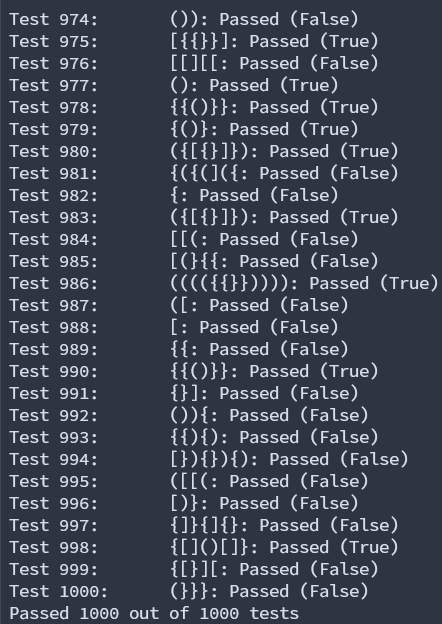
\includegraphics{Qn2_testing}
\end{figure}
\subsection{Invalid Inputs}
Invalid inputs are a superset of valid inputs, thus the selection of brackets to insert at any given point is expanded to include all invalid closing brackets as well. The generator then selects a random index \(i\) to insert random brackets until the max length is reached. Then, the generator checks if the number of opening brackets match the number of closing brackets for each type of bracket. If they match, a random index is selected again to either insert or remove a bracket. This ensures that we also deal with the case that the length of the input string is odd. The generator then provides the input string and whether the string is valid to a checker function, which compares the output of the developed algorithm with the validity of the input string. To run the tests, a user may run |python test.py --tests \{number of tests\} --length \{max length of input strings\}|. The output will show how many tests the algorithm passes, and what the generated input strings were for each test.
\section{Listings}
\subsection{Algorithm}
\begin{lstlisting}[language=Python]
	import re

	def main(statement:str):
		return is_balanced(statement)

	def is_balanced(statement:str) -> bool:
		bracket_pairing = {
			"{": "}",
			"[": "]",
			"(": ")"
		}
		# fast check
		statement = re.sub(r"[A-Za-z0-9\*\-\+\^\/\=]", "", statement)
		if len(statement) % 2 != 0: return False
		brackets = [bracket for bracket in bracket_pairing.keys()]\
			+ [bracket for bracket in bracket_pairing.values()]
		stack = [ ]
		for char in statement:
			if char in brackets:
				if char in bracket_pairing.keys():
					stack.append(char)
				else:
					try:
						if bracket_pairing[stack.pop()] != char:
							return False
					except IndexError:
						return False
		return len(stack) == 0

	if __name__ == "__main__":
		res = main(input("Enter an algebraic statement: "))
		print(res)
\end{lstlisting}
\subsection{Testing}
\begin{lstlisting}[language=Python]
	import argparse
	import random
	from main import is_balanced

	def test_is_balanced(iters: int, max_length:int=10):
		"""Tests the is_balanced function over a given number of iterations.

		Args:
			iters (int): number of iterations
		"""
		results = []
		for i in range(iters):
			statement, proper = statement_generator(random.randint(1, max_length))
			print(f"Test {i+1}:\t{statement}:", end=" ")
			res = is_balanced(statement)
			if res == proper:
				print(f"Passed ({res})")
			else:
				print(f"Failed: {res} (should be {proper})")
			results.append(res == proper)
		print(f"Passed {results.count(True)} out of {iters} tests")

	def statement_generator(length: int):
		"""Generates a random algebraic statement of a given length.

		Args:
			length (int): length of the statement

		Returns:
			str: random algebraic statement
		"""
		length //= 2
		bracket_pairing = {
			"{": "}",
			"[": "]",
			"(": ")"
		}
		brackets = [bracket for bracket in bracket_pairing.keys()]\
			+ [bracket for bracket in bracket_pairing.values()]
		ret = ""
		state = random.choice([True, False])
		ret += random.choice([bracket for bracket in bracket_pairing.keys()])
		stack = [ret[0]]
		for _ in range(length):
			if state:
				candidates = [b for b in bracket_pairing.keys()]
				if ret[-1] in bracket_pairing.keys():
					candidates += [bracket_pairing[ret[-1]]]
				ret += random.choice(candidates)
				if ret[-1] in bracket_pairing.values():
					stack.pop()
				else:
					stack.append(ret[-1])
			else:
				ret += random.choice(brackets)
		for _ in range(len(stack)):
			if state:
				ret += bracket_pairing[stack.pop()]
			else:
				ret += random.choice(brackets)
		if not state:
			n_additions = random.randint(0, length)
			insertion_index = random.randint(0, len(ret))
			additions = [random.choice(brackets) for _ in range(n_additions)]
			ret = ret[:insertion_index-1] + "".join(additions) + ret[insertion_index+1:len(ret)+1-n_additions]
			# count the number of bracket pairs
			bracket_counts = {(k, v): 0 for k, v in bracket_pairing.items()}
			for char in ret:
				for k, v in bracket_pairing.items():
					if char == k:
						bracket_counts[(k, v)] += 1
					elif char == v:
						bracket_counts[(k, v)] -= 1
			# if the statement is potentially balanced, either remove or add a random character.
			if all([count == 0 for count in bracket_counts.values()]):
				# remove a random character
				if len(ret) > 2:
					loc = random.randint(1, len(ret)-1)
					ret = ret[:loc] + ret[loc+1:]
				else:
					ret += random.choice(brackets)
		return (ret, state)

	def main(tests: int=1000, max_length:int=10):
		test_is_balanced(tests, max_length)

	if __name__ == "__main__":
		parser = argparse.ArgumentParser()
		parser.add_argument("-t", "--tests", type=int, default=1000, help="number of tests to run")
		parser.add_argument("-l", "--length", type=int, default=10, help="maximum length of the statement")
		args = parser.parse_args()
		main(args.tests, args.length)
\end{lstlisting}
\chapter{}
\section{Problem Statement}
Write an array-based implementation of the array list ADT that achieves \(\mathcal{O}(1)\) time for insertion and removals at the front and at the end of the array list. Your implementation should also provide for an \(\mathcal{O}(1)\) time |get(i)| method. Assume that overflow does not occur. Explain and justify why your implementation has achieved the stated time complexity requirements.
\section{Requirements/Specification}
The program creates an array list with functions to insert and remove items at the front and back of the array as well as a function |get(i)| to get the element in the array at index |i|.

The function |insertItem(int input, int position)| inserts an item into the array. The argument input will be the item and the argument position will decide where the item will be inserted into the array. If the position is 0, the item will be inserted at the front of the array. If the position is 1, the item will be inserted at the end of the array. For example, |insertItem(15, 1)| will insert the item |15| at the end of the array.

The function |removeItem(int position)| removes an item from the array. The argument position will decide whether the item will be removed from the start or from the end of the array. If the position is 0, the item at the start of the array will be removed. If the position is 1, the item at the end of the array will be removed. For example, |removeItem(0)| will remove the item at the start of the array.
\section{User Guide}
\section{Structure/Design}
The program starts by creating an array with a large size (e.g. |int arr[100];|) and variables start (e.g. |int start = 50;|) and end (e.g. |int end = 51;|) to represent the starting and ending index of the array respectively. The array will be initialised somewhere in the middle of the array with the start index and end index next to each other. The array is between the start and end index of the array which will then expand or contract from there depending on where the items are inserted or removed (at the front or at the back of the array).
\begin{figure}[H]
	\centering
	\caption{Initialising the array}
	\begin{tikzpicture}[MyStyle/.style={draw, minimum width=2em, minimum height=2em, outer sep=0pt}]
		\matrix (A) [matrix of math nodes, nodes={MyStyle, anchor=center}, column sep=-\pgflinewidth]{ \phantom{1} & \cdots & \phantom{1} & \phantom{1} & \phantom{1} & \phantom{1} & \phantom{1} & \phantom{1} & \phantom{1} & \phantom{1} & \phantom{1} & \cdots & \phantom{1} \\};
		\node[below=of A-1-7] (start) {start};
		\node[below=of A-1-8] (end) {end};
		\draw[->] (start.north) to (A-1-7.south);
		\draw[->] (end.north) to (A-1-8.south);
	\end{tikzpicture}
	\label{fig:qn3_init}
\end{figure}
To add an item at the start of the array, the start position of the array will first take in the value of the item, then the start index will shift left (i.e. |start--;|). Similarly, to add an item at the end of the array, the end position of the array will take in the value of the item, then the end index will shift right (i.e. |end++;|). Since the function does not need to iterate through the array to insert the items, the time complexity for inserting items is \(\mathcal{O}(1)\).

\begin{figure}[H]
	\centering
	\caption{Insertion}
	\begin{tikzpicture}[MyStyle/.style={draw, minimum width=2em, minimum height=2em, outer sep=0pt}]
		\matrix (A) [matrix of math nodes, nodes={MyStyle, anchor=center}, column sep=-\pgflinewidth]{ \phantom{1} & \cdots & \phantom{1} & \phantom{1} & \phantom{1} & \phantom{1} & 7 & \phantom{1} & \phantom{1} & \phantom{1} & \phantom{1} & \cdots & \phantom{1} \\};
		\node[below=of A-1-6] (start) {start};
		\node[below=of A-1-8] (end) {end};
		\draw[->] (start.north) to (A-1-6.south);
		\draw[->] (end.north) to (A-1-8.south);
	\end{tikzpicture}
	\label{fig:qn3_insert}
\end{figure}
Even though the problem statement assumes that overflow does not occur, safety measures were put in place to prevent overflowing. If the start index is at the start of the array (i.e. |start == 0|) or the end index is at the end of the array (i.e. |end == 99|), trying to add another item into the array will print “Overflow!”

To remove an item from the start of the array, the start index will simply shift right (i.e. |start++;|), and to remove an item from the end of the array, the end index will simply shift left (i.e. |end--;|). Since the function only shifts the start or end index when removing items and does not iterate through the array, the time complexity for removing items is \(\mathcal{O}(1)\).
\begin{figure}[H]
	\centering
	\caption{Removal of nodes}
	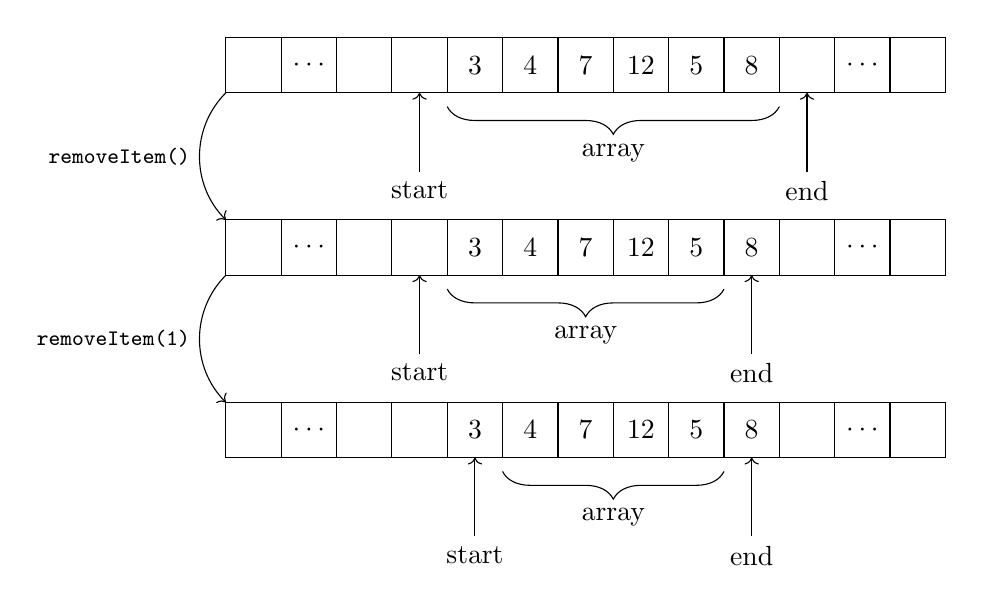
\begin{tikzpicture}[MyStyle/.style={draw, minimum width=2em, minimum height=2em, outer sep=0pt}]
		\matrix (A) [matrix of math nodes, nodes={MyStyle, anchor=center}, column sep=-\pgflinewidth]{ \phantom{1} & \cdots & \phantom{1} & \phantom{1} & 3 & 4 & 7 & 12 & 5 & 8 & \phantom{1} & \cdots & \phantom{1} \\};
		\node[below=of A-1-4] (start) {start};
		\node[below=of A-1-11] (end) {end};
		\draw[->] (start.north) to (A-1-4.south);
		\draw[->] (end.north) to (A-1-11.south);
		\draw[decorate, decoration={brace, amplitude=10pt, raise=5pt, mirror}](A-1-5.south west) to node[black, midway, below=15pt] {array} (A-1-10.south east);
		\matrix (B) [matrix of math nodes, nodes={MyStyle, anchor=center}, column sep=-\pgflinewidth, below=of A, yshift=-10pt]{ \phantom{1} & \cdots & \phantom{1} & \phantom{1} & 3 & 4 & 7 & 12 & 5 & 8 & \phantom{1} & \cdots & \phantom{1} \\};
		\node[below=of B-1-4] (start) {start};
		\node[below=of B-1-10] (end) {end};
		\draw[->] (start.north) to (B-1-4.south);
		\draw[->] (end.north) to (B-1-10.south);
		\draw[decorate, decoration={brace, amplitude=10pt, raise=5pt, mirror}](B-1-5.south west) to node[black, midway, below=15pt] {array} (B-1-9.south east);
		\draw[->] (A-1-1.south west) to [bend right=45] node[midway, left] {\texttt{\footnotesize removeItem()}} (B-1-1.north west);
		\matrix (C) [matrix of math nodes, nodes={MyStyle, anchor=center}, column sep=-\pgflinewidth, below=of B, yshift=-10pt]{ \phantom{1} & \cdots & \phantom{1} & \phantom{1} & 3 & 4 & 7 & 12 & 5 & 8 & \phantom{1} & \cdots & \phantom{1} \\};
		\node[below=of C-1-5] (start) {start};
		\node[below=of C-1-10] (end) {end};
		\draw[->] (start.north) to (C-1-5.south);
		\draw[->] (end.north) to (C-1-10.south);
		\draw[decorate, decoration={brace, amplitude=10pt, raise=5pt, mirror}](C-1-6.south west) to node[black, midway, below=15pt] {array} (C-1-9.south east);
		\draw[->] (B-1-1.south west) to [bend right=45] node[midway, left] {\texttt{\footnotesize removeItem(1)}} (C-1-1.north west);
	\end{tikzpicture}
	\label{fig:qn3_remove}
\end{figure}
The array is deemed empty when the start and end index are next to each other. When a function is called to remove another item while the array is empty, it will print ``List is empty!''.

To get the item at index |i| of the array, the function starts counting at the start of the array (i.e. |arr[start + 1]|) and returns the item at index i of the array (i.e. |arr[start + 1 + i]|). Since this function returns the item at the stated index and does not require iteration through the array, the time complexity for this function is \(\mathcal{O}(1)\).

\begin{figure}[H]
	\centering
	\caption{List access example (accessing index 4)}
	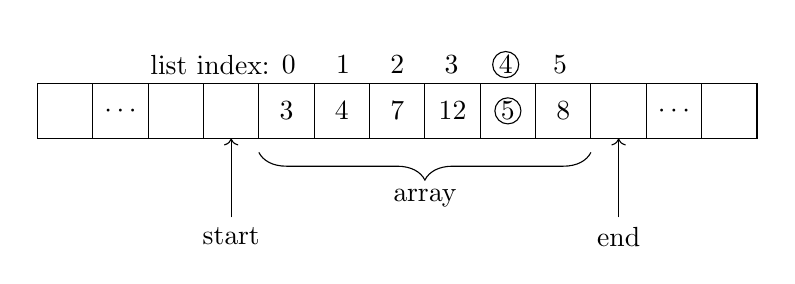
\begin{tikzpicture}[MyStyle/.style={draw, minimum width=2em, minimum height=2em, outer sep=0pt}]
		\matrix (A) [matrix of math nodes, nodes={MyStyle, anchor=center}, column sep=-\pgflinewidth]{ \phantom{1} & \cdots & \phantom{1} & \phantom{1} & 3 & 4 & 7 & 12 & 5 & 8 & \phantom{1} & \cdots & \phantom{1} \\};
		\node[below=of A-1-4] (start) {start};
		\node[below=of A-1-11] (end) {end};
		\draw[->] (start.north) to (A-1-4.south);
		\draw[->] (end.north) to (A-1-11.south);
		\draw[decorate, decoration={brace, amplitude=10pt, raise=5pt, mirror}](A-1-5.south west) to node[black, midway, below=15pt] {array} (A-1-10.south east);
		\matrix (B) [matrix of math nodes, nodes={minimum width=2em, minimum height=2em, outer sep=0pt, anchor=center, above of=A, yshift=15pt}, column sep=-\pgflinewidth]{ \phantom{1} & \phantom{\cdots} & \phantom{1} & \phantom{1} & 0 & 1 & 2 & 3 & 4 & 5 & \phantom{1} & \phantom{\cdots} & \phantom{1} \\};
		\node[left of=B-1-5] {list index:};
		\node[circle, draw] at (A-1-9) {};
		\node[circle, draw] at (B-1-9) {};
	\end{tikzpicture}
	\label{fig:qn3_access}
\end{figure}
\section{Limitations}
The limitation of this array list ADT is that it has a maximum size depending on the value used during initialization and has a finite number of items that can be added into the array. The function only stops the list from overflowing, but it does not have a solution to overflowing (e.g.\ increasing the size of the array).
\section{Testing}
Testing is handled by the |main()| function in the program. Initially, the array is empty.

First, the program tests the |insertItem()| function by adding elements to the start and end of the array. Adding an item to an invalid position will output |``Invalid Input!''|.
\begin{figure}[H]
	\centering
	\caption{insertItem() testing}
	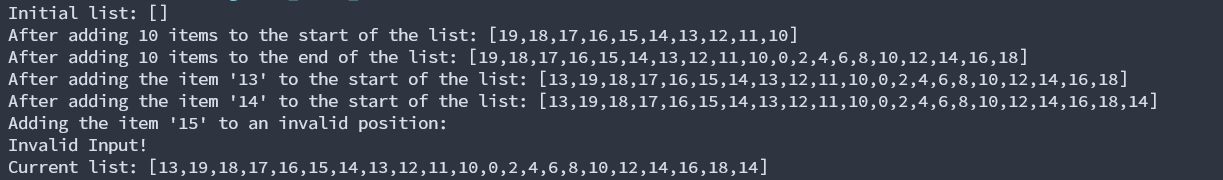
\includegraphics[width=0.8\textwidth]{qn3_test1}
	\label{fig:qn3_insertitem}
\end{figure}

Next, the program tests the |removeItem()| function by removing an item at the start and at the end of the array. Removing an item at an invalid location will output |``Invalid Input!''|.
\begin{figure}[H]
	\centering
	\caption{removeItem() testing}
	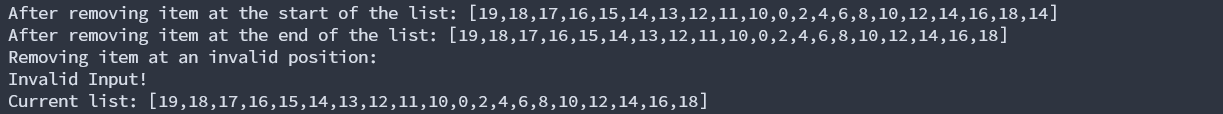
\includegraphics[width=0.8\textwidth]{qn3_test2}
	\label{fig:qn3_removeitem}
\end{figure}

Thirdly, the program tests the |get()| function at index |5|. Using an out of range index will output |``Index Out Of Range!''|.
\begin{figure}[H]
	\centering
	\caption{get() testing}
	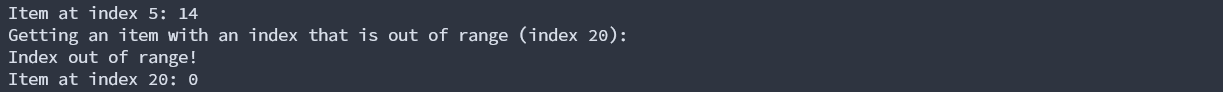
\includegraphics[width=0.8\textwidth]{qn3_test3}
	\label{fig:qn3_get}
\end{figure}

Subsequently, the program will attempt to overflow the array at the start and end. The program will then output ``Overflow!'' when items cannot be added to that respective position any more.
\begin{figure}[H]
	\centering
	\caption{Overflow testing}
	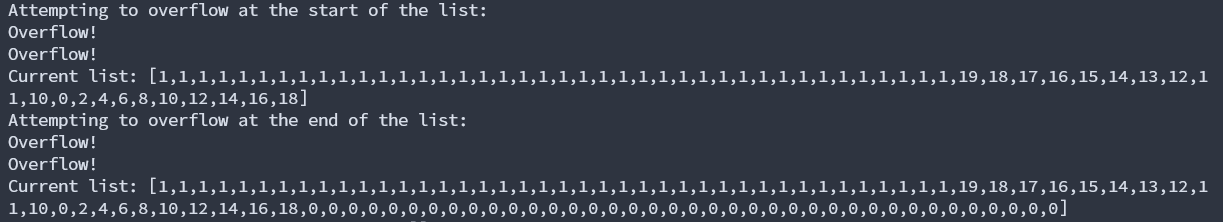
\includegraphics[width=0.8\textwidth]{qn3_test4}
	\label{fig:qn3_overflow}
\end{figure}

Lastly, the program will remove every item in the array to empty the array. Then, it will attempt to remove an item from the empty array, which will output |``List is empty!''|. This concludes the testing.
\begin{figure}[H]
	\centering
	\caption{Empty array removeItem() testing}
	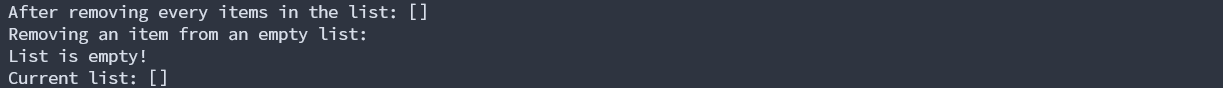
\includegraphics[width=0.8\textwidth]{qn3_test5}
	\label{fig:qn3_emptyarray}
\end{figure}
\section{Listings}
\begin{lstlisting}[language=C]
	#include <stdio.h>

	int arr[100];
	int start = 50;
	int end = 51;

	int insertItem(int input, int position) {   // position: 0 for inserting at the front; 1 for inserting at the end
		if (position == 0) {
			if (start == 0) {
				printf("Overflow!\n");
			}
			else {
				arr[start] = input;
				start--;
			}
		}
		else if (position == 1) {
			if (end == 99) {
				printf("Overflow!\n");
			}
			else {
				arr[end] = input;
				end++;
			}
		}
		else {
			printf("Invalid Input!\n");
		}
	}

	int removeItem(int position) {              // position: 0 for removing at the front; 1 for removing at the end
		if (end - start == 1) {
			printf("List is empty!\n");
			return 0;
		}
		if (position == 0) {
			start++;
		}
		else if (position == 1) {
			end--;
		}
		else {
			printf("Invalid Input!\n");
		}
	}

	int get(int i) {                            // get(i) returns the item in the list at index i
		if (i >= 0 && i < end - start - 1) {
			return arr[start + 1 + i];
			
		}
		else {
			printf("Index out of range!\n");
			return NULL;
		}
	}

	int printList() {
		printf("[");
		for (int i = 0; i < end - start - 2; i++) {
			printf("%d,", arr[start + 1 + i]);
		}
		if (end - start == 1) {
			printf("]\n");
		}
		else {
			printf("%d]\n", arr[end - 1]);
		}
	}

	int main() {
		// initial list
		printf("Initial list: ");
		printList();

		// inserting 10 items to the start of the list
		for (int i = 0; i < 10; i++) {
			insertItem(i + 10, 0);
		}
		printf("After adding 10 items to the start of the list: ");
		printList();

		// inserting 10 items to the end of the list
		for (int i = 0; i < 10; i++) {
			insertItem(i * 2, 1);
		}
		printf("After adding 10 items to the end of the list: ");
		printList();

		// inserting the item '13' at the start of the list
		insertItem(13, 0);
		printf("After adding the item '13' to the start of the list: ");
		printList();

		// inserting the item '14' at the end of the list
		insertItem(14, 1);
		printf("After adding the item '14' to the start of the list: ");
		printList();

		// inserting the item '15' at an invalid position
		printf("Adding the item '15' to an invalid position:\n");
		insertItem(15, 2);
		printf("Current list: ");
		printList();

		// removing the item at the start of the list
		removeItem(0);
		printf("After removing item at the start of the list: ");
		printList();

		// removing the item at the end of the list
		removeItem(1);
		printf("After removing item at the end of the list: ");
		printList();

		// removing the item at an invalid position
		printf("Removing item at an invalid position:\n");
		removeItem(2);
		printf("Current list: ");
		printList();

		// get the item at index 5 of the list
		printf("Item at index 5: %d\n", get(5));

		// get the item at index 20 of the list
		printf("Getting an item with an index that is out of range (index 20):\n");
		printf("Item at index 20: %d\n", get(20));

		// attempting to overflow at the start of the list
		printf("Attempting to overflow at the start of the list:\n");
		for (int i = 0; i < 42; i++) {
			insertItem(1, 0);
		}
		printf("Current list: ");
		printList();

		// attempting to overflow at the end of the list
		printf("Attempting to overflow at the end of the list:\n");
		for (int i = 0; i < 40; i++) {
			insertItem(0, 1);
		}
		printf("Current list: ");
		printList();

		// removing all the items in the list
		for (int i = 0; i < 98; i++) {
			removeItem(1);
		}
		printf("After removing every items in the list: ");
		printList();

		// attempting to remove an item from an empty list
		printf("Removing an item from an empty list:\n");
		removeItem(1);
		printf("Current list: ");
		printList();
}
\end{lstlisting}
\chapter{}
\section{Problem Statement}
Write a recursive algorithm to check that a sentence is a palindrome (ignoring blanks, lower case and upper case differences, and punctuation marks, so that ``Madam, I'm Adam'' is accepted as a palindrome). Analyse the efficiency of your implementation and provided a detailed discussion of its time complexity.
\ex{}{Please enter a sentence: Madam, I'm Adam Check if ``Madam, I'm Adam'' is a palindrome: True}
\section{Requirements/Specification}
This program is supposed to compare the characters in the sentence. First and last, Second and second last etc. If it matches, it is a palindrome. Some assumptions/conditions would be ignoring blanks, lower case, upper case differences, and punctuation marks. Some assumptions/conditions would be ignoring blanks, lower case, upper case differences, and punctuation marks. Empty strings will be considered as a palindrome too.
\section{User Guide}
\begin{enumerate}
	\item Click on the ``Run'' button in the IDE to run the program with python. Alternatively, running |python <filename>.py| will run the program.
	\item Input a sentence when prompted in the command line interface.
	\item The resulting output will show whether the input sentence was a palindrome.
\end{enumerate}
\section{Structure/Design}
The design of the system is that it will remove all punctuations and black spaces in the string then change all uppercase characters to lowercase characters before passing through the |palindrome| function. After the system has recorded the new string, a function for |palindrome| and |isPalindrome| will run to check the string and determine whether it is a palindrome.

For the |palindrome| function, if there is only one character it will return |true|. If the first and last characters do not match, it will return |false|. For more than 2 characters, it will check the middle substring whether the characters match.

For the |isPalindrome| function, if it is an empty string, it will be considered a palindrome and return |true|.

The operation of removing punctuations and blanks, and converting the string to lowercase is \(\mathcal{O}(n)\), \(n\) being the length of the string. As it iterates through the function |palindrome|, it checks if the first and last characters match, hence the time complexity of this function is \(\mathcal{O}(n)\). The function |isPalindrome| checks if the string is empty, hence the time complexity of the entire algorithm is \(\mathcal{O}(n)\).

\section{Limitations}
The algorithm assumes an ASCII input, thus input strings with extended UTF-8 encoding may result in erroneous output.
\section{Testing}
From the |main.py| file, users are able to manually input a string they would like to check and if the string is a palindrome, it will return True. However, when the user inputs invalid inputs such as string that is not a palindrome, it will return False.
\begin{figure}[H]
	\centering
	\caption{Valid and invalid inputs}
	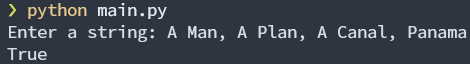
\includegraphics[width=0.4\textwidth]{qn4_input}
	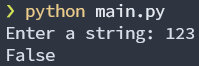
\includegraphics[width=0.175\textwidth]{qn4_invalid}
	\label{fig:qn4_input}
\end{figure}
From the |test.py| file, the input strings are generated randomly with 50\% being palindromes. The user can set the arguments |-i| and |-l| to set the number of tests and max generated string length (ASCII letters only) respectively. ASCII symbols are generated in between ASCII letters in order to test the filtering capabilities of the algorithm. An example output of running the testing script is shown in~\autoref{fig:qn4_test}.
\begin{figure}[H]
	\centering
	\caption{Running the testing script}
	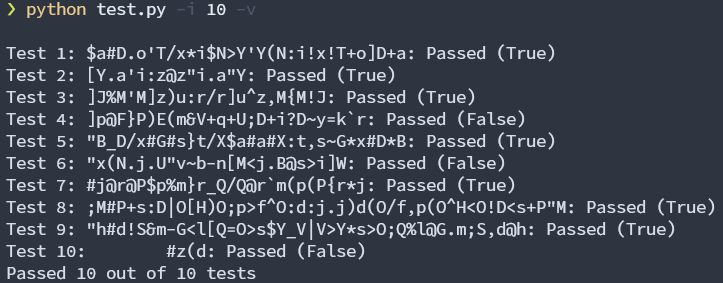
\includegraphics[width=0.8\textwidth]{qn4_test}
	\label{fig:qn4_test}
\end{figure}

\section{Listings}
\subsection{Algorithm}
\begin{lstlisting}[language=python]
	def main():
		# user input for string
		input_str = input("Enter a string: ")
		# Output
		if isPalindrome(input_str):
			print("True")
		else:
			print("False")

	def palindrome(str2, s, e):
		# If there is only one character
		if (s == e):
			return True

		# If first and last characters do not match
		if (str2[s] != str2[e]):
			return False

		# for > 2 characters, checking for middle substring
		if (s < e + 1):
			return palindrome(str2, s + 1, e - 1)
		return True

	# for empty string, it will be considered as palindrome too
	def isPalindrome(input_str):
		
		# remove all punctuations and blank spaces
		str2 = ''.join(i for i in input_str if i.isalnum())
		# lower uppercase characters
		str2 = str2.lower()
		n = len(str2)

		if n == 0:
			return True
		return palindrome(str2, 0, n - 1)
	if __name__ == "__main__":
		main()
\end{lstlisting}
\subsection{Testing}
\begin{lstlisting}[language=python]
	import argparse
	import random
	import string

	from main import isPalindrome

	def string_generator(length: int, is_palindrome: bool):
		half_length = length // 2
		odd = length % 2
		letter = string.ascii_letters
		generated_string = ''.join(random.choice(letter) for i in range(length))
		if is_palindrome:
			half = generated_string[:half_length + odd][::-1]
			generated_string = generated_string[:half_length + odd] + half
		elif generated_string[0].lower() == generated_string[-1].lower():
			generated_string += random.choice([i for i in letter if i.lower() != generated_string[0].lower()])
		elif len(generated_string) == 1:
			generated_string += random.choice([i for i in letter if i.lower() != generated_string[0].lower()])
		symbols = string.punctuation
		generated_string = ''.join(random.choice(symbols) + i for i in generated_string)
		return generated_string

	def test_is_palindrome(iters: int, max_length: int=10, verbose: bool=False, hackerman: bool=False):
		"""Tests the isPalindrome function over a given number of iterations.

		Args:
			iters (int): number of iterations
		"""
		results = []
		if hackerman:
			end = '\x1b[2K\r'
		else:
			end = "\n"
		i = 0
		while True:
			test_state = random.choice([True, False])
			generated_string = string_generator(random.randint(1, max_length), test_state)
			res = isPalindrome(generated_string)
			p = ""
			if verbose or res != test_state:
				print(f"{end}Test {i+1}:\t{generated_string}:", end=" ")
			if res == test_state:
				p = f"Passed ({res})" if verbose else ""
			else:
				p = f"Failed: {res} (should be {test_state})"
			if len(p):
				print(f"{p:<50}", end="")
			results.append(res == test_state)
			i += 1
			if i == iters:
				break
		print(f"{end}Passed {results.count(True)} out of {iters} tests")

	if __name__ == "__main__":
		parser = argparse.ArgumentParser(description="Test the isPalindrome function")
		parser.add_argument("-i", "--iters", type=int, default=100000, help="number of iterations")
		parser.add_argument("-l", "--length", type=int, default=25, help="maximum length of the string")
		parser.add_argument("-v", "--verbose", action="store_true", help="verbose mode")
		parser.add_argument("-H", "--hackerman", action="store_true", help="hackerman mode")
		args = parser.parse_args()
		test_is_palindrome(args.iters, args.length, args.verbose, args.hackerman)
\end{lstlisting}
\chapter{}
\section{Problem Statement}
\begin{enumerate}[label=(\alph*)]
	\item Explain the meaning of stability in a sorting algorithm.
	\item Explain a situation why stability in sorting is desired.
	\item State which algorithms are stable. Prove it with an implementation of a stable and an unstable sorting algorithm. Discuss in detail your justification.
	\begin{enumerate}[label=\roman*.]
		\item Selection sort
		\item Insertion sort
		\item Quick sort
	\end{enumerate}
\end{enumerate}
\solve{
	\begin{enumerate}[label=(\alph*)]
		\item Stability refers to whether a sorting algorithm respects the relative positions of elements with equal values during the sort. An unstable sorting algorithm would not preserve the order of elements with equal values.
		\item One situation could be where there is a line of people queueing who need to be ordered by age. If there are two people standing in line whoa re the same age, a stable sort will ensure that the order of the person who arrived first will stay the same.
		\item All three algorithms can have stable and unstable implementations.
	\end{enumerate}
}
\section{Requirements/Specification}
The program implements python code for selection, insertion and quick sort algorithms. In order to clearly demonstrate the stability of each algorithm, the program will accept an unsorted list of 2-element tuples, where the first element is a unique identifier for the tuple and the second element is the value that is compared against other values for the sorting algorithms. Some example inputs are: |[("a", 3), ("b", 3)]|, |[["a", 3], ["b", 3]]|, and |[[123, 3], [456, 3]]|.
\section{User Guide}
The program can be run from the command line with |python <filename>.py|. Since the assignment requires a proof by implementation, the input data has been pre-defined in the script. If a user would like to input their own data, they may do so by changing the following variables accordingly.
\begin{itemize}
	\item |data_selection| -- for selection sort
	\item |data_insertion| -- for insertion sort
	\item |data_quick| -- for quick sort
\end{itemize}
\section{Structure/Design}
The code for all 3 sorting algorithms are contained in functions, so for a user to see the sorting processes, they would have to call each sorting algorithm's respective functions. All 3 sorts will print the elements in the array during each iteration of the sort.
\section{Limitations}
As the program uses tuples to demonstrate the stability of the algorithms, the program will not take in any other formats like simple lists as input. For instance, |[26, 54, 56, 32]| and |["a", "b", "c"]| are not valid inputs.
\section{Testing}
The stability of the algorithm may be demonstrated by showing the unsorted input array and how it is iteratively sorted until the algorithm outputs the sorted array. For the arrays used to test the algorithms, two elements are declared with equal value, with the first of the pair having a `first' identifier, and the second having a `second' identifier. This will allow users to track the relative positions of these two elements of equal value. The output of the python script is shown in~\autoref{fig:qn5_output}.
\begin{figure}[H]
	\centering
	\caption{Outputs of stable and unstable variants of the sorting algorithms}
	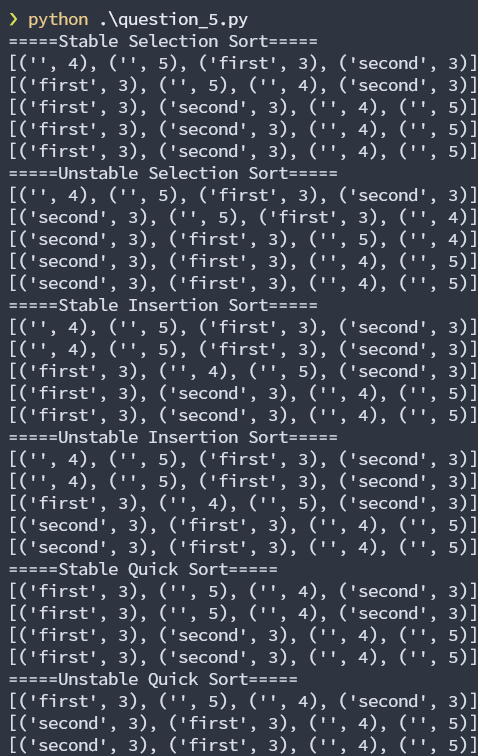
\includegraphics[width=0.8\textwidth]{qn5_output}
	\label{fig:qn5_output}
\end{figure}
\section{Listings}
\begin{lstlisting}[language=python]
	#Function for selection sort (Stable)
	def selectionSort(array, size, stable=True):
		for ind in range(size):
			min_index = ind

			if stable:
				for j in range(ind + 1, size):
					# select the minimum element in every iteration
					if array[j][1] < array[min_index][1]:
						min_index = j
			else:
				for j in range(size - 1, ind, -1):
					if array[j][1] < array[min_index][1]:
						min_index = j
			# swapping the elements to sort the array
			(array[ind], array[min_index]) = (array[min_index], array[ind])
			print(array)

	# Function to do insertion sort (Stable)
	def insertionSort(arr, stable=True):
		# Traverse through 1 to len(arr)
		for i in range(1, len(arr)):

			key = arr[i]
			# Move elements of arr[0..i-1], that are
			# greater than key, to one position ahead
			# of their current position
			j = i-1
			if stable:
				while j >= 0 and key[1] < arr[j][1]:
					arr[j + 1] = arr[j]
					j -= 1
				arr[j + 1] = key
			else:
				while j >= 0 and key[1] <= arr[j][1]:
					arr[j + 1] = arr[j]
					j -= 1
				arr[j + 1] = key
			print(arr)
		return arr

	# Python program for implementation of Quicksort Sort (Stable)
	# Function to find the partition position
	def partition(array, low, high, stable=True):

		# choose the rightmost element as pivot
		if stable:
			pivot = array[high][1]
		else:
			pivot = array[low][1]

		# pointer for greater element
		i = low - 1

		# traverse through all elements
		# compare each element with pivot
		for j in range(low, high):
			if (stable and array[j][1] <= pivot) or (not stable and array[j][1] < pivot):
				# If element smaller than pivot is found
				# swap it with the greater element pointed by i
				i += 1
				# Swapping element at i with element at j
				(array[i], array[j]) = (array[j], array[i])
				print(array)
		# Swap the pivot element with the greater element specified by i
		(array[i + 1], array[high]) = (array[high], array[i + 1])
		# Return the position from where partition is done
		return i + 1

	# function to perform quicksort
	def quickSort(array, low, high, stable=True):
		if low < high:

			# Find pivot element such that
			# element smaller than pivot are on the left
			# element greater than pivot are on the right
			pi = partition(array, low, high, stable)

			# Recursive call on the left of pivot
			quickSort(array, low, pi - 1)

			# Recursive call on the right of pivot
			quickSort(array, pi + 1, high)

	data_selection = [("", 4), ("", 5), ("first", 3), ("second", 3)]
	#print("Unsorted Array: ", data_selection)
	print("=====Stable Selection Sort=====")
	print(data_selection)
	size = len(data_selection)
	selectionSort(data_selection, size)

	data_selection = [("", 4), ("", 5), ("first", 3), ("second", 3)]
	print("=====Unstable Selection Sort=====")
	size = len(data_selection)
	print(data_selection)
	selectionSort(data_selection, size, False)

	print("=====Stable Insertion Sort=====")
	data_insertion = [("", 4), ("", 5), ("first", 3), ("second", 3)]
	print(data_insertion)
	print(insertionSort(data_insertion))

	print("=====Unstable Insertion Sort=====")
	data_insertion = [("", 4), ("", 5), ("first", 3), ("second", 3)]
	print(data_insertion)
	print(insertionSort(data_insertion, False))

	print("=====Stable Quick Sort=====")
	data_quick = [("first", 3), ("", 5), ("", 4), ("second", 3)]
	print(data_quick)
	quickSort(data_quick, 0, len(data_quick) - 1)
	print(data_quick)

	print("=====Unstable Quick Sort=====")
	data_quick = [("first", 3), ("", 5), ("", 4), ("second", 3)]
	print(data_quick)
	quickSort(data_quick, 0, len(data_quick) - 1, False)
	print(data_quick)
\end{lstlisting}
\end{document}
